%% AAAI-27 anonymous submission: single-tool-use evaluation paper.
%% SCAFFOLD ONLY: sections are empty (TODO pointers, no prose). See GOALS.md for scope.
%% Full formatting rules: authorkit27/AnonymousSubmission2027.pdf
%% Preamble below is the AAAI-27 kit preamble verbatim. DO NOT CHANGE the marked lines.

\documentclass[letterpaper]{article} % DO NOT CHANGE THIS
\usepackage[submission]{aaai2027}  % DO NOT CHANGE THIS  (anonymous submission mode)
% Fonts are loaded automatically by aaai2027.sty (newtxtext, helvet, courier).
% DO NOT add \usepackage{times}, {helvet}, {courier}, or any other font package.
\usepackage[hyphens]{url}  % DO NOT CHANGE THIS
\usepackage{graphicx} % DO NOT CHANGE THIS
\urlstyle{rm} % DO NOT CHANGE THIS
\def\UrlFont{\rm}  % DO NOT CHANGE THIS
\usepackage{natbib}  % DO NOT CHANGE THIS AND DO NOT ADD ANY OPTIONS TO IT
\usepackage{caption} % DO NOT CHANGE THIS AND DO NOT ADD ANY OPTIONS TO IT
\frenchspacing  % DO NOT CHANGE THIS

% Recommended for algorithms (remove if unused before final submission).
\usepackage{algorithm}
\usepackage{algorithmic}

% Recommended for listings, e.g. PDDL snippets (remove if unused before final submission).
\usepackage{newfloat}
\usepackage{listings}
\DeclareCaptionStyle{ruled}{labelfont=normalfont,labelsep=colon,strut=off} % DO NOT CHANGE THIS
\lstset{%
	basicstyle={\footnotesize\ttfamily},
	numbers=left,numberstyle=\footnotesize,xleftmargin=2em,
	aboveskip=0pt,belowskip=0pt,
	showstringspaces=false,tabsize=2,breaklines=true}
\floatstyle{ruled}
\newfloat{listing}{tb}{lst}{}
\floatname{listing}{Listing}

% Recommended for better-looking tables.
\usepackage{booktabs}

% amsmath for \text in the P(call) x P(correct|call) decomposition notation.
\usepackage{amsmath}

\pdfinfo{
/TemplateVersion (2027.1)
}

\setcounter{secnumdepth}{0} % 0 = unnumbered sections (AAAI default). Set to 1/2 to number.

% ============================ Title & Authors ============================
% Title is NOT anonymized (only authors are). Title Case (Chicago) required.
\title{Availability Is Not Enough: When Symbolic Tools Help---and Hurt---LLMs on Planning Tasks}

% Anonymous submission: sole "author" is "Anonymous Submission"; affiliations empty.
% De-anonymize (real authors/affiliations) only at camera-ready via CameraReady2027.tex.
\author{
    Anonymous Submission
}
\affiliations{
    %
}

\newif\ifaddcomments
\addcommentstrue % Uncomment this line to remove the user comments

\newcommand{\commentout}[1]{ }

\newcommand{\todo}[1]{\ifaddcomments{\textcolor{red}{[TODO: #1]}}\fi}
\newcommand{\roni}[1]{\ifaddcomments{\textcolor{orange}{[Roni: #1]}}\fi}
\newcommand{\yarin}[1]{\ifaddcomments{\textcolor{violet}{[Yarin: #1]}}\fi}
\newcommand{\shahaf}[1]{\ifaddcomments{\textcolor{blue}{[Shahaf: #1]}}\fi}
\newcommand{\omer}[1]
{\ifaddcomments{\textcolor{teal}{[Omer: #1]}}\fi}

% Censoring bounds (indeterminate trials counted both ways). Typographically
% distinct from Wilson intervals [a, b] by design; see the Metrics subsection.
\newcommand{\cbnd}[2]{\ensuremath{\langle #1,\,#2\rangle}}

\begin{document}

\maketitle

\begin{abstract}
Sound symbolic planners and validators are correct by construction, and language
models are increasingly able to call them as tools. But does access actually help
an LLM on planning tasks, and when? Using PDDL as a setting where a deterministic
oracle can grade every answer exactly, we evaluate five single-tool-use tasks
(solving, domain, problem, and plan validation, and state-trajectory simulation)
across five open-weight models and two frontier models, grading every tool-arm
trial twice: at the answer the model \emph{delivers}, our primary surface, and at
the tool results it obtained along the way, the mechanism layer. A three-arm
design separates tool \emph{availability}
from a one-sentence \emph{steering} nudge, every proportion carries a confidence
interval or an explicit censoring bound, and a signed-significance rule
distinguishes help from harm. The benefit
is strongly regime-dependent. Solving is transformed wherever the unaided model
is floored ($8$--$29\%$ across tiers; $95\%$ delivered with the tool at the
frontier); the validation tasks are lifted over weak baselines, one rescued from
below its trivial majority guess. What limits the rest is two behaviors distinct
from capability and from tool accuracy. The first is invocation: on plan
checking, one of three $\geq$9B models stops calling the validator when it is
merely \emph{available} (its tool path drops $67$\,pp) and reasons in prose
instead, and one steering sentence moves invocation from $21\%$ to $94\%$, with
the tool $>$99\% accurate when called. The second is delivery: what the tool
verifies often fails to reach the final answer, by an amount that grows with
answer length (nothing on verdicts, five points on plans, tens of points on
state trajectories), the same at both frontier tiers. Measured in tokens, the
tool pays for itself
where the model cannot do the task unaided. The pattern holds under reasoning mode
and an anonymized-domain contamination control.
\end{abstract}

% Optional anonymized links block (uncomment near submission; do NOT de-anonymize).
% \begin{links}
%     \link{Code}{...}
%     \link{Datasets}{...}
% \end{links}

\section{Introduction}
% DRAFT 2026-06-14 (goal 1, partial).
% Findings preview must match Results; no "first" claims.
Large language models are increasingly deployed as agents that call external
tools, and automated planning is an unusually clean setting in which to ask
whether that helps. Decades of research have produced planners and validators that
are \emph{correct by construction}: a plan a sound solver returns provably reaches
the goal, and a verdict a sound validator issues is sound
\citep{helmert2006fastdownward, howey2004val}. If a language model can simply
\emph{call} such a tool, it should be able to offload the parts of a PDDL
task (search, state tracking, and plan checking) on which language models are
known to be unreliable \citep{valmeekam2023planbench, kambhampati2024llmmodulo}.
Whether this actually improves end-to-end performance, when it does, and at
what cost, is the question we study.

The question is less settled than it may appear. One line of work tests LLMs
\emph{as} planners and finds they fall well short of solvers
\citep{valmeekam2023planbench}; a second uses LLMs as \emph{formalizers} that
translate language into PDDL for a downstream solver
\citep{liu2023llmp, tantakoun2025survey}; and a third measures tool-use competence
in isolation, without a planning oracle \citep{bfcl2025}. The specific question,
whether access to a sound PDDL tool improves a model across the planning task
pipeline measured end-to-end, has not been answered cleanly. A credible answer
requires controlling for several confounds at once: whether the model is even
prompted to use the tool, whether the baseline is floored or already competent,
reasoning-mode (extended-thinking) decode budgets, and contamination of public
benchmark domains. This paper sets out to do exactly that, grading $4{,}560$
trials per model-mode-arm cell strictly end-to-end against a solver oracle rather
than by tool \emph{selection}, with a confidence interval on every proportion and
an anonymized-domain control for memorization.

We evaluate five single-tool-use PDDL tasks (\emph{solve}, \emph{validate\_domain},
\emph{validate\_problem}, \emph{validate\_plan}, \emph{simulate}) across five
open-weight models (from the Qwen and Gemma families), grading every response strictly against a deterministic
solver/validator oracle rather than by self-report. A three-arm design separates
tool \emph{availability} (the tool is present) from a one-sentence \emph{steering}
nudge (the model is told to use it), every proportion carries a confidence
interval, and verdicts use a signed-significance rule that distinguishes a tool
that helps from one that hurts. A separate sweep over anonymized domains controls
for contamination, and a token cost-of-pass analysis asks what the tool is worth
per correct answer.

The benefit is strongly regime-dependent rather than uniform. Of the
five tasks, two (\emph{solve}, \emph{simulate}) essentially do not happen
unaided under the deployed budget and format constraints; on two (\emph{validate\_domain}, \emph{validate\_problem}) the tool
improves over weak baselines, one of them genuinely partial and the other at or
below the trivial majority guess. What limits the rest is two behaviors distinct
from capability and from tool accuracy. On \emph{validate\_plan}, merely making
the tool available collapses one $\geq$9B model's validator invocation to $21\%$
of trials (its tool path drops $67$\,pp) as it reasons in prose instead, and a
single steering sentence repairs the invocation; and across tasks, what the tool
verifies inside the trial often fails to reach the model's final answer, a
\emph{delivery gap} that grows with answer length and persists at the frontier
tier. Where the unaided
baseline has headroom, the tool's advantage grows with plan length; it is
cost-effective in tokens where the model cannot do the task unaided; and the
pattern survives reasoning mode and an anonymized-domain control. We make the
following contributions:
\begin{itemize}
\item A controlled three-arm, five-task evaluation of symbolic PDDL
tool utility over five open-weight and two frontier models, graded at two
labeled layers (the delivered answer as the primary surface; the tool's verified
result as the mechanism layer), with confidence intervals, explicit censoring
bounds where storage truncated answers, and a
signed-significance verdict rule that separates help from harm.
\item The identification of
\emph{invocation propensity} (a large, unstable, prompt- and mode-dependent free
variable, rather than capability or tool accuracy) as the factor that limits the
tool path:
it factors as $P(\text{call})\times P(\text{correct}\mid\text{call})$, with
nearly all between-arm, between-model, and cross-mode variance living in the first
factor, and for a model that under-calls, mere \emph{availability} collapses the
tool path on a task it already does well, a failure one steering sentence
reverses.
\item The measurement of the \emph{delivery gap} between what the tool verifies
and what the model's answer contains: near zero on verdict-length answers,
$+5.0$\,pp on plans, and tens of points on state trajectories, identical at two
frontier tiers, so the gap tracks answer length rather than model strength.
\item A token cost-of-pass analysis showing the tool pays for itself where the
unaided baseline is floored, and is a luxury where it is already strong.
\item Robustness evidence: the verdict pattern reproduces under reasoning mode
through budget-insensitive statistics, and an anonymized-domain contamination
probe returns null.
\end{itemize}

\section{Background and Related Work}
% DRAFT 2026-06-14 (goal 2). Re-derived for our framework.

Automated planning studies how to find a sequence of actions that turns an
initial state into one that satisfies a goal. The Planning Domain Definition Language (PDDL)
\citep{mcdermott1998pddl, fox2003pddl21} is the field's standard formalism, and decades of
research have produced sound, complete solvers such as Fast Downward
\citep{helmert2006fastdownward} and FF \citep{hoffmann2001ff} for classical planning and
ENHSP \citep{scala2016enhsp} for numeric planning, together with plan validators such as
VAL \citep{howey2004val}. These systems are correct by construction: a plan they return
provably reaches the goal, and a verdict they issue is sound. They are, however, brittle to
the formal-modelling step: a domain or problem must be expressed in precise PDDL before
any solver can run. Where a model must reason in the solver's place, numeric domains are the
harder regime: tracking arithmetic effects on continuous fluents adds to the discrete
state-tracking that language models already struggle with.

\subsection{Large Language Models for Planning}
Large language models have been probed extensively as planners. Systematic benchmarks show
that, prompted to produce plans directly, even strong LLMs fall well short of solver-level
reliability \citep{valmeekam2023planbench}. \citet{kambhampati2024llmmodulo} argue from this
evidence that autoregressive LLMs cannot plan or self-verify on their own, and propose
\emph{LLM-Modulo} frameworks in which the model is paired with external, model-based
verifiers that supply the soundness it lacks. The present study is empirical evidence for
exactly this division of labour: we measure what an LLM gains when a sound planner or
validator is available as a callable tool, rather than asking the model to be the planner.

\subsection{Large Language Models as Planning Formalizers}
A complementary line treats the LLM not as the planner but as a \emph{formalizer} that
translates natural language into PDDL, delegating search to a sound solver. LLM+P
\citep{liu2023llmp} pipelines an LLM into a classical planner; \citet{guan2023world} use
LLMs to construct world models for model-based planning; Plansformer
\citep{pallagani2022plansformer} fine-tunes for plan generation; and pretrained LLMs have
been applied to generalized planning in PDDL domains \citep{silver2024generalized}.
\citet{tantakoun2025survey} survey this rapidly growing ``LLMs-as-formalizers'' area (where the consensus is that pairing
an LLM translator with a sound solver outperforms end-to-end LLM planning), and
\citet{huang2025limit} characterize its limits, showing that although models are largely robust to
lexical perturbation of domain symbols, formalization quality degrades as natural-language
descriptions move away from templated phrasing. Their work is also the published starting
point for our PlanBench section. They show that writing PDDL and handing it to a solver
rescues an obfuscated domain where direct planning scores nothing, at $70$ of $100$
against $0$ of $100$ for GPT-4o, graded with VAL. We repeat that result and add the
control it was missing (Section~\ref{sec:planbench}). \citet{lamalfa2026endtoend} report
the closest agentic system, where end-to-end PDDL planning agents raise PlanBench
averages by about $15$ points over $3$ runs of $50$ instances per task. This literature largely studies the \emph{generation} of
PDDL, evaluated on a single downstream question (does the produced model solve?). We instead
evaluate LLMs \emph{using} planning and validation tools across five distinct PDDL tasks,
with strict end-to-end grading against a solver oracle.

\subsection{Tool Use, Agent Protocols, and Their Evaluation}
Equipping LLMs with external tools is now standard, from learned tool invocation
\citep{schick2023toolformer} to large API repertoires \citep{qin2024toolllm}. The Model
Context Protocol \citep[MCP;][]{anthropic2024mcp} standardizes how tools are described and
called (in practice a vendor-neutral schema for exposing functions and their argument types to a
model and relaying the model's invocations), and is the mechanism by which we expose planners and
validators to the model. A
growing body of benchmarks measures tool-use competence: single-turn function calling
\citep{bfcl2025} and multi-turn tool-agent-user interaction \citep{yao2024taubench}, among
others. A parallel line raises invocation through scaffolding rather than measuring it,
interleaving reasoning with tool actions \citep{yao2023react} or offloading numeric
subproblems to executable programs \citep{chen2023pot}. Our setting sits deliberately at the simple end of this spectrum: each task admits
exactly one relevant, correct-by-construction tool, so the appropriate analog is single-call
function selection rather than long-horizon orchestration. We use this point to calibrate
our results.

\subsection{Positioning}
Across these three lines, LLMs are studied \emph{as} planners
\citep{valmeekam2023planbench}, \emph{as} formalizers that emit PDDL for a downstream
solver \citep{liu2023llmp, tantakoun2025survey}, or for tool-use competence in isolation
\citep{bfcl2025}; none measures what a model gains when a sound planner or validator is
available as a callable tool across the full set of PDDL tasks, graded end-to-end against
the solver itself. That is the gap we close. This paper contributes a controlled evaluation
of whether such symbolic tools help LLMs: five single-tool-use PDDL tasks across five
models, a three-arm design that separates tool \emph{availability} from a one-sentence
steering \emph{nudge}, confidence intervals with signed significance, a contamination
control over anonymized domains, and a token-cost (cost-of-pass) analysis. We then carry
a smaller version of the design onto PlanBench \citep{valmeekam2023planbench}, where the
prompts are plain English and the model has to write the PDDL itself. That section
re-measures the no-tools baseline against the published figures and tests the tool effect
against a control that keeps the same prompt and removes only the tools
(Section~\ref{sec:planbench}).

\section{Methodology}
We ask a single, deliberately narrow question: \emph{when a sound symbolic
planner or validator is available as a callable tool, how much does it improve a
language model's performance on individual PDDL tasks, and at what token cost?}
The study crosses five PDDL tasks, five open-weight models, two reasoning modes,
and three experimental arms, and grades every response strictly against a
deterministic solver/validator oracle rather than by self-report.

\subsection{Experimental Pipeline}
A single evaluation harness turns the fixture corpus into graded trials, and every
(model, reasoning mode, arm) cell runs the same four stages. In \emph{setup}, the
harness loads the PDDL domain corpus and connects to the symbolic tools over the
Model Context Protocol \citep{anthropic2024mcp}. In the \emph{oracle} stage, before
any model is queried, an oracle calls those tools directly on every fixture to
produce ground truth (a reference plan, a validity verdict, or a state trajectory,
according to the task); a startup check re-confirms each fixture against its
committed label and aborts the run on any drift. During \emph{trials}, for each
task, paraphrase, and instance the harness builds the prompt, serves the model with
vLLM at temperature~0, and in the tool arms lets it issue up to ten tool calls
before it commits a final answer, logging that answer with its token counts and any
tool calls. Finally, \emph{grading} scores each response strictly against the oracle
(Table~\ref{tab:tasks}), tags it by failure mode, and aggregates it into a success
rate with a Wilson \citep{wilson1927} score interval. The rest of this section
details each stage: the tool suite the model calls, the tasks and fixtures, model
serving, the three arms, and the statistics.

\subsection{The Tool Suite}
The tools the model may call are a suite of sound symbolic planners and
validators, each exposed as a Model Context Protocol \citep{anthropic2024mcp}
function with a typed argument schema and reached through a single
natural-language entry point: the model reads a task description, selects a tool,
emits a structured call, and receives the tool's result. Five tools cover the
five tasks. A classical and a numeric planner (Fast Downward
\citep{helmert2006fastdownward} and ENHSP \citep{scala2016enhsp}) return a plan
for \emph{solve}; three validators built on the \texttt{unified-planning} library
issue VALID/INVALID verdicts for \emph{validate\_domain}, \emph{validate\_problem},
and \emph{validate\_plan}; and a state-transition tool returns the full trajectory
a plan induces for \emph{simulate}. Every tool is sound and deterministic, so a
correctly formed call is correct by construction; what the model contributes is
recognizing which tool a task needs and invoking it with well-typed arguments. The
suite packages the Planning Copilot tools of \citet{benyamin2025copilot}, whose
evaluation covered the same five task types with $250$ single-task queries in
total ($10$ problems, $5$ prompt variants, $5$ request types); the corpus graded
here runs $4{,}560$ trials in every model-mode-arm cell, about $18$ times that
entire suite per cell. The
verbatim per-task prompts that expose these tools, together with the one-sentence
steering directive, appear in Listing~\ref{lst:prompts}.

\subsection{Tasks, Oracle, and Fixtures}
Each model is given five PDDL tasks, one tool-relevant per task: \emph{solve}
(find a plan reaching the goal), \emph{validate\_domain} and
\emph{validate\_problem} (judge whether a domain or problem file is well formed),
\emph{validate\_plan} (judge whether a given plan is correct), and
\emph{simulate} (produce the full state trajectory a plan induces, action by
action). Before any model is run, an oracle generates ground truth by calling
these same tools directly. The one deterministic toolchain both defines ground
truth and, in the tool arms, is what the model may call, so a correctly invoked
tool is correct by construction; what the experiment measures is therefore
whether and how the model invokes the tool, not the tool's own accuracy. Grading is end-to-end and
strict (Table~\ref{tab:tasks}): a \emph{solve} answer counts only if the
returned plan is independently certified valid; a \emph{simulate} answer counts
only if its entire trajectory equals the oracle's under a canonical normal form
(sorted, case-folded, with the boolean/numeric fluent shapes unified), with no
partial credit and no free-text fallback. Both arms are graded on the model's own
final message, by the same parser; a tool arm's trial is \emph{additionally}
scored at a diagnostic layer from the tool's returned result on the model's
arguments, which attests correct selection and faithful invocation. The Metrics
subsection defines the two layers and fixes the delivered answer as the primary
surface (models essentially never contradict the tool, so where the layers
disagree the cause is an answer that never restated the result, not one that
misreported it).

\begin{table}[t]
\centering
\footnotesize
\begin{tabular}{@{}lp{0.62\columnwidth}@{}}
\toprule
\textbf{Task} & \textbf{Graded correct iff (vs.\ deterministic oracle)} \\
\midrule
solve            & returned plan is certified valid (goal reached, all preconditions hold) \\
validate\_domain & VALID/INVALID verdict matches the oracle \\
validate\_problem & verdict matches the oracle \\
validate\_plan   & verdict matches the oracle \\
simulate         & full state trajectory equals the oracle's (canonical form; no partial credit) \\
\bottomrule
\end{tabular}
\caption{The five single-tool-use tasks and their strict success criteria. Each
task has a single relevant, correct-by-construction tool per instance
(\emph{solve} selects the classical or numeric planner).}
\label{tab:tasks}
\end{table}

The fixture corpus is 20 PDDL domains: 10 classical (e.g., blocksworld,
gripper, rovers, satellite, depots) and 10 numeric (e.g., counters, farmland,
sailing, drone), assembled from standard planning domains and public benchmark
suites. Each domain ships
matched valid and mutated-invalid files so the verdict tasks score against both
positive and negative instances (balanced one-to-one for \emph{validate\_problem}
and \emph{validate\_plan}; \emph{validate\_domain} carries a $5{:}1$
positive-to-negative ratio, which widens its negative-arm interval). Every committed positive is
re-validated and every negative is confirmed rejected at startup, so a fixture
that drifts from its label aborts the run. Holding model, reasoning mode, and arm
fixed, one cell comprises 4{,}560 graded trials: \emph{solve} 300,
\emph{validate\_domain} 360, \emph{validate\_problem} 600, \emph{validate\_plan}
3{,}000, and \emph{simulate} 300. Each cell spans three neutral paraphrases per
task (imperative, declarative, interrogative framings), a linguistic-robustness
probe; the steering directive introduced below is held byte-identical across the
three, isolating steering variance from paraphrase variance.

\subsection{Models and Serving}
We evaluate five open-weight instruction-tuned models spanning over an order of
magnitude in scale (0.8B--35B) and two families: Qwen3.5-0.8B, Qwen3.5-4B, Qwen3.5-9B,
a Gemma mixture-of-experts model ($\approx$26B total / $\approx$4B active
parameters, ``Gemma-MoE-26B''), and Qwen3.6-35B.\footnote{Hugging Face checkpoints:
\texttt{Qwen/Qwen3.5-0.8B}, \texttt{Qwen/Qwen3.5-4B}, and
\texttt{Qwen/Qwen3.5-9B}, served in 16-bit precision; the two
mixture-of-experts checkpoints, \texttt{cyankiwi/gemma-4-26B-A4B-it-AWQ-4bit}
and \texttt{cyankiwi/Qwen3.6-35B-A3B-AWQ-4bit}, are community AWQ-INT4
quantizations.} Headline conclusions are drawn
from the three larger models ($\geq$9B: Qwen3.5-9B, Gemma-MoE-26B,
Qwen3.6-35B); the 4B model is reported for scaling context and the 0.8B model
isolates a small-model failure mode (Results). All models are served locally with
vLLM (CUDA on Linux) on single $48$\,GB and $96$\,GB GPUs, one model per GPU and with
server-side prefix caching enabled.\todo{Pin exact vLLM/CUDA/NVIDIA-driver/OS versions
once the experiment suite is final: record them here and flip the ``computing
infrastructure'' Reproducibility Checklist item from \emph{partial} to \emph{yes}.}
Decoding is deterministic
(temperature~0), so each trial is a single fixed sample and the confidence
intervals we report quantify sampling uncertainty over the fixture instances
(treated as the inferential population), not decoding stochasticity, which
temperature~0 removes.
The context window is 16{,}384 tokens; per-task decode caps are 8{,}192 tokens for
\emph{solve} and 6{,}144 for the others; tool-using runs may iterate up to ten
tool calls. In practice tool use is overwhelmingly single-shot: across the $91{,}200$
with-tools trials the median trial issues one call, and $60\%$ issue exactly one (of
which $90\%$ succeed). The $27\%$ that issue two or more are retries after an
unsuccessful call, and their success rate falls monotonically as call count rises
($67\%$ at two calls to ${\approx}25\%$ beyond five). A further $13\%$ issue no call at
all, the silent failures dissected in Results. Capping at a single call would
therefore remove low-yield retries rather than successes. The reasoning mode is toggled per run (\emph{think}~=~on/off via the
serving runtime's thinking switch). Under \emph{think}~=~on the
reasoning trace and the final answer share the \emph{same} per-task decode cap, a
shared budget that drives the confound we treat explicitly below. Tools are
exposed to the model through the Model Context Protocol \citep{anthropic2024mcp}
as standard function definitions; system prompts are thin per-task policy stubs,
with all argument schemas carried by the tool definitions rather than the prompt.

\subsection{The Three-Arm Design}
Every (model, mode, task) is run in three primary arms (a fourth, control arm
follows); arms are scored separately and never pooled, and every comparison is
between two arms of the \emph{same} cell:
\begin{itemize}
\item \textbf{no-tools}: the model answers from parametric knowledge. The PDDL
tools are removed, but per-task JSON-schema-constrained decoding remains, so the
baseline is not held back by formatting alone; only the symbolic tools are absent.
\item \textbf{tool-available (plain)}: the \emph{byte-identical} neutral task
prompt, now with the tools exposed. (The thin per-task system prompts are structural
mirrors sharing the same role-framing first sentence and sentence count. They differ
in their policy clause, ``use the available tool'' vs.\ ``use your own reasoning,''
the latter adding an output-format reminder on the verdict tasks; we revisit this
small instruction-surface difference in Limitations.) Differencing this arm
against no-tools yields the \emph{availability gap}, which isolates tool presence.
\item \textbf{tool-steered}: the neutral prompt plus exactly one appended
sentence directing the model to use the tool. Differencing against the plain arm
yields the \emph{steering gap}.
\end{itemize}

Listing~\ref{lst:prompts} gives the verbatim text for these three arms: the
no-tools and tool-available \emph{validate\_plan} system prompts (representative;
the four other stubs swap in the matching tool name) and the one-sentence
steering directive for every task. The complete prompt bank ships with the
released harness.

\begin{listing}[t]
\begin{lstlisting}
validate_plan, no-tools (system prompt):
  You are a PDDL validation assistant. PDDL validation tools
  are not available in this evaluation. Analyze whether the
  plan solves the problem using your own reasoning; end your
  response with exactly one line: VERDICT: VALID or VERDICT:
  INVALID.

validate_plan, tool-available (system prompt):
  You are a PDDL validation assistant. LLMs cannot reliably
  check plan correctness from training alone. Use the
  available validation tool to check whether the plan solves
  the problem.

steering directive (appended to the neutral user prompt):
  solve:            Use the planner tool with the domain and
                    problem as arguments.
  validate_domain:  Use the validate_domain tool with the
                    domain as its argument.
  validate_problem: Use the validate_problem tool with the
                    domain and problem as arguments.
  validate_plan:    Use the validate_plan tool with the
                    domain, problem, and plan as arguments.
  simulate:         Use the get_state_transition tool with the
                    domain, problem, and plan as arguments.
\end{lstlisting}
\caption{The thin per-task policy stubs. The availability contrast differences the
no-tools and tool-available system prompts (which differ by the policy clause); the
steering contrast appends the single directive shown to the neutral user prompt (the
only difference between the plain and steered arms).}
\label{lst:prompts}
\end{listing}

The two contrasts map onto the function-calling literature: the plain arm
measures \emph{relevance detection} (does the model spontaneously invoke the
right tool when its existence is known but not urged?) and the steered arm
measures \emph{function selection} (told to use a tool, does it pick the correct
one?) in the sense of the Berkeley Function-Calling Leaderboard
\citep{bfcl2025}. Because the per-task tool split enforces each tool's required
arguments through its schema, argument-filling errors are largely structural, so
the steered contrast isolates selection rather than parameter construction.
A fourth, \emph{control} arm (the steering directive with the tools still
removed) tests whether the directive alone moves the no-tools floor; it is
reported as a control, not a primary outcome. The \emph{realizable benefit} of
the tool, used as the cross-mode spine below, is success(tool-steered)
$-$ success(no-tools): what a deployment that actually prompts for tool use would
realize.

\subsection{Metrics, Confidence Intervals, and Signed Significance}
\paragraph{One primary surface, two layers.} The primary outcome on every task,
in every arm, is the \emph{delivered} success rate: the answer in the model's own
final message is graded against the deterministic oracle, by the same parser in
both arms. This is the surface a user of the system experiences; a correct result
that the model obtained from a tool but never carried into its answer does not
count. In the tool arms we grade each trial at a second, diagnostic layer as
well: \emph{tool-verified} success asks whether a correct result appeared in some
tool response during the trial, whatever the final message then said. The two
layers separate the mechanism (did the model drive the tool to a correct
result?) from the outcome (did that result reach the answer?), and their
difference is itself a measurement, the \emph{delivery gap}. Tool-verified
numbers are never headlines; wherever one appears below it is labeled as the
mechanism layer. One boundary case gets its own outcome category: a trial whose
final message is empty although a correct tool result exists earlier in the
transcript is \emph{delegation-terminal}. The strict rule grades it as a
failure, since the answer never reached the user; crediting such trials instead
would move $3.6\%$ of tool-arm rows and flips no headline verdict.

\paragraph{One surface, three value shapes.} Our corpora differ in how much of
the final message was stored, and the reported value shape follows the storage,
not the estimand. Where the full text is available the delivered rate is an
exact point with a Wilson 95\% interval, written $[a,\,b]$. Where responses were
stored as truncated snapshots, a snapshot that ends before any verdict is
visible leaves the trial \emph{indeterminate}: it cannot be graded correct or
incorrect. Cells containing indeterminate trials are reported as censoring
bounds, written \cbnd{a}{b}: the delivered rate lies between ``every
indeterminate trial failed'' ($a$) and ``every indeterminate trial succeeded''
($b$). The two notations are typographically distinct on purpose and are never
mixed in one cell. A claim that involves a bounded cell is asserted only if it
survives the claim-adverse end of every bound involved (with the Wilson interval
then placed on that end), and cells where the indeterminate mass could flip the
call are stated as \emph{undecided} rather than resolved. This heterogeneity of
shapes is itself evidence about protocol design: full-response storage buys
exactness, and Results opens with a table saying which corpus bought it.

In the tool arms we additionally record \emph{tool\_selected} (whether the model
called the task-matching tool at all); tool calls and their results are stored
in full in every corpus, so invocation rates and tool-verified rates are exact
everywhere, whatever the final-answer storage. Failures are typed
(tool not selected, wrong tool, verdict mismatch, unparseable output, trajectory
mismatch), with cap-truncated responses re-tagged as truncations rather than
being counted as content failures. Every reported proportion carries a Wilson 95\%
score interval \citep{wilson1927}, and \emph{arms are never pooled}: each statistic comes from
exactly one (model, mode, arm) corpus, and only differences \emph{between} such
statistics are formed. Because each instance is scored under three paraphrases,
trials within an instance are not independent: the intraclass correlation is
$\approx$0.6 and the design effect $\approx$2.2--2.7, so the effective sample size is
roughly half the nominal count and these Wilson intervals are correspondingly
anti-conservative. We verified that every headline verdict ($+50$--$92$\,pp, and the
smallest reported gaps) remains CI-disjoint after inflating intervals by
$\sqrt{2.7}$, and flag the one verdict-relevant gap that does not (the $-5$\,pp
\emph{validate\_problem} steering dip) individually. As a robustness check on the largest
verdict-relevant contrast, we additionally fit an instance-level random-intercept logistic model to
the Gemma-MoE \emph{validate\_plan} plain-vs-steered comparison (success $0.206\!\to\!0.926$); the
steering effect is strongly favorable and significant (log-odds $+7.5$, posterior SD $0.10$; a
population-averaged GEE with an exchangeable working correlation clustered on instance agrees), so
the verdict is invariant to whether non-independence is handled by design-effect inflation or by an
explicit random-effects model. We do not fit such models cell-by-cell because many cells are
near-degenerate or completely separated (the \emph{simulate} no-tools baseline is $0/3{,}000$,
and the tool arms reach $P(\text{correct}\mid\text{call})\!\approx\!0.99$), where a
maximum-likelihood GLMM is undefined or unstable, whereas the design-effect inflation never fits a
per-cell model and so remains valid at the boundary; with cluster size three the random-effect
variance is also only weakly identified.

Verdicts use a \emph{signed} significance rule. A per-model gap counts as
favorable evidence only when the two arms' 95\% intervals are disjoint
\emph{and} the gap points the hypothesized way (the tool helps); a disjoint gap
pointing the other way is tallied separately as significant-\emph{against}, which
we treat as a finding in its own right. A research question reads \textsc{yes} when favorable
significant gaps dominate with none against, \textsc{mixed} when significant
against-gaps are present, and \textsc{no} when no significant favorable movement
exists. This sign-awareness carries real weight: on \emph{validate\_plan} mere tool
availability collapses one $\geq$9B model's validator invocation to $21\%$ of
trials, a mechanism-layer drop of $-67$\,pp in tool-verified success, and a
sign-blind disjointness test would credit that highly significant movement as
the tool ``having an effect.'' The signed rule reads it as evidence against. Requiring disjoint 95\% intervals is deliberately
conservative: it controls the false-positive rate well below $\alpha=0.05$, at
the cost of power on small gaps, so a \textsc{no} verdict means ``no movement we
are willing to call significant,'' not ``no movement.'' We do not apply a separate family-wise
correction across cells, but the headline verdicts are not thereby exposed to
multiplicity. The design-effect inflation already widens every interval by
$\sqrt{2.7}$, so a gap is called significant only when its arms are disjoint at an
effective $z\approx3.2$ rather than the nominal $1.96$; that threshold is already
stricter than a Bonferroni bound for a confirmatory family as large as ${\sim}30$
contrasts (Bonferroni $z\approx3.1$), so the verdicts clear simultaneous control
without a dedicated correction. The reported effects are moreover large, and we
treat the few borderline gaps as exploratory rather than confirmatory.

\subsection{Cross-Mode Aggregation and the Robust Floor}
\emph{think}~=~off is the clean headline: the model answers directly, so the
availability and steering gaps measure the tool, unconfounded. Under
\emph{think}~=~on the shared decode budget truncates a large fraction of $\geq$9B
no-tools trials (the baseline uses up its decode budget on reasoning), so raw
\emph{think}~=~on gaps conflate the tool's value with baseline budget collapse.
We therefore make cross-mode claims only through budget-insensitive statistics.
The spine is the realizable benefit (steered, not plain: under
\emph{think}~=~on the plain arm largely stops calling the tool, so its
availability gap also includes a mode-dependent tool-calling failure that
steering repairs). Gaps carry Newcombe MOVER intervals \citep{newcombe1998}, and the mode difference
$\Delta(\mathrm{on}-\mathrm{off})$ carries a MOVER interval for the difference of two
independent gaps, valid because the two reasoning-mode corpora share no
trials. The \emph{robust floor} is the minimum realizable benefit over the two
reasoning modes (the smaller of the two mode point estimates, a deliberately
conservative construction): a lower bound that neither mode's decode budget can inflate.
Against a deliberately conservative $+30$\,pp threshold this sorts the tasks into
\emph{robust} (every $\geq$9B floor $\geq +30$\,pp), \emph{sole-source} (baseline at
$0$ in both modes, where a benefit with no baseline cannot be budget-confounded), and
\emph{budget-dependent} (some floor below $+30$\,pp, where the large
\emph{think}~=~on stretch is the artifact).

\subsection{Contamination Control}
Because the domains are public, an unaided baseline could be inflated by
memorization. A separate sweep re-ran the entire matrix on structurally identical
domains with every surface symbol (domain, predicate, and object names) renamed.
Under \emph{think}~=~off the clean no-tools probe is near-null (mean
$|\Delta(\mathrm{canonical}-\mathrm{anonymized})|$ success $1.1$\,pp, max $3.7$, with zero
CI-disjoint task cells), so where the baseline has headroom it carries no
detectable memorization signal, and the availability gap (tool arm minus this
clean baseline) therefore cannot be a contamination artifact on the baseline
side. The only CI-disjoint cells appeared under \emph{think}~=~on and
trace to tokenization rather than memory: the renamed prompts ran $\approx$5\% longer,
so more trials truncated under the shared budget while success-given-completion
was unchanged. This is itself a live demonstration of the budget confound the
cross-mode analysis controls for.

\section{Results}
% Delivered-surface reframe (D-J2, 2026-09-07). Open-roster delivered numbers come
% from results/derived/e2e_overlay/pooled_e2e_table.csv; verdicts from
% development/job2_delivered_reframe_worknote.md. Mechanism-layer (tool-verified)
% numbers keep the locked deck values (checkpoints/rq-sweep5v2/).
Unless stated otherwise, every figure is \emph{think}~=~off (the unconfounded
read) on the three $\geq$9B models, with reasoning mode treated separately in the
Robustness subsection. All headline rates are \emph{delivered} (Methodology): the
model's own final answer graded against the oracle, with tool-verified rates
appearing only as the labeled mechanism layer. The \emph{availability} gap is
+tool(plain)~$-$~no-tools and the \emph{steering} gap is
+tool(steered)~$-$~+tool(plain), each significant when the two arms' 95\%
intervals are disjoint; where a cell is a censoring bound \cbnd{a}{b}, the gap is
asserted only if it survives the claim-adverse end. Table~\ref{tab:howtoread}
says, for each corpus, which value shape its delivered rates take and why, and
its footnotes list the claims this discipline forbids; we recommend reading it
before any table below. Figure~\ref{fig:funnel} draws the same discipline for
every with-tools cell that can be drawn: of all trials, how many call the tool,
how many obtain a correct tool result, and how many deliver a correct answer,
against the unaided rate as a reference line.

\begin{table*}[t]
\centering
\footnotesize
\begin{tabular}{@{}p{0.26\textwidth}p{0.20\textwidth}p{0.13\textwidth}p{0.31\textwidth}@{}}
\toprule
\textbf{Corpus (arms)} & \textbf{Final-answer storage} & \textbf{Delivered shape} & \textbf{What it can support} \\
\midrule
Open-weight sweeps, canonical $+$ anonymized (no-tools arm) & full text at grading
time & exact $[a,\,b]$; \emph{simulate} \cbnd{a}{b} & unaided baselines; the
contamination null \\
Open-weight sweeps (tool arms) & $500$-char snapshot & bounds \cbnd{a}{b} &
availability and steering verdicts at claim-adverse bounds; straddling cells stay
\emph{undecided} \\
Frontier runs, Claude Haiku~4.5 $+$ Sonnet~4.6 (both arms) & $16$K snapshot;
no-tools de-censored from raw batch output & exact, except \emph{simulate}
\cbnd{a}{b} & exact delivered lifts and the delivery gap at two capability tiers \\
Independent full-storage rerun (tool arms, \emph{think}=on, reasoning parser off)
& full text & exact or near-exact & separate-apparatus replication;
\emph{within}-corpus contrasts only \\
Budget-decoupled control (no-tools) & full text & exact & the unaided-capability
question only \\
\bottomrule
\end{tabular}
\caption{How to read our numbers: one primary surface (delivered), three value
shapes, fixed by what each corpus stored. Wilson 95\% intervals print as
$[a,\,b]$; censoring bounds print as \cbnd{a}{b} and are never resolved by
optimism. Four claims are ruled out by construction and do not appear in this
paper: (i) no delivered-vs-tool-verified gap is computed across corpora, only
within one; (ii) an undecided open-roster cell is never resolved by importing the
full-storage rerun, whose job-level parity with the main sweep failed (it is a
replication under a different apparatus, not a repair); (iii) no claim that tools
are the sole source of \emph{simulate} success is made at the delivered level;
(iv) the rerun's \emph{solve} cells carry a known parser-off truncation shift and
are excluded from headline use.}
\label{tab:howtoread}
\end{table*}

\begin{figure*}[t]
\centering
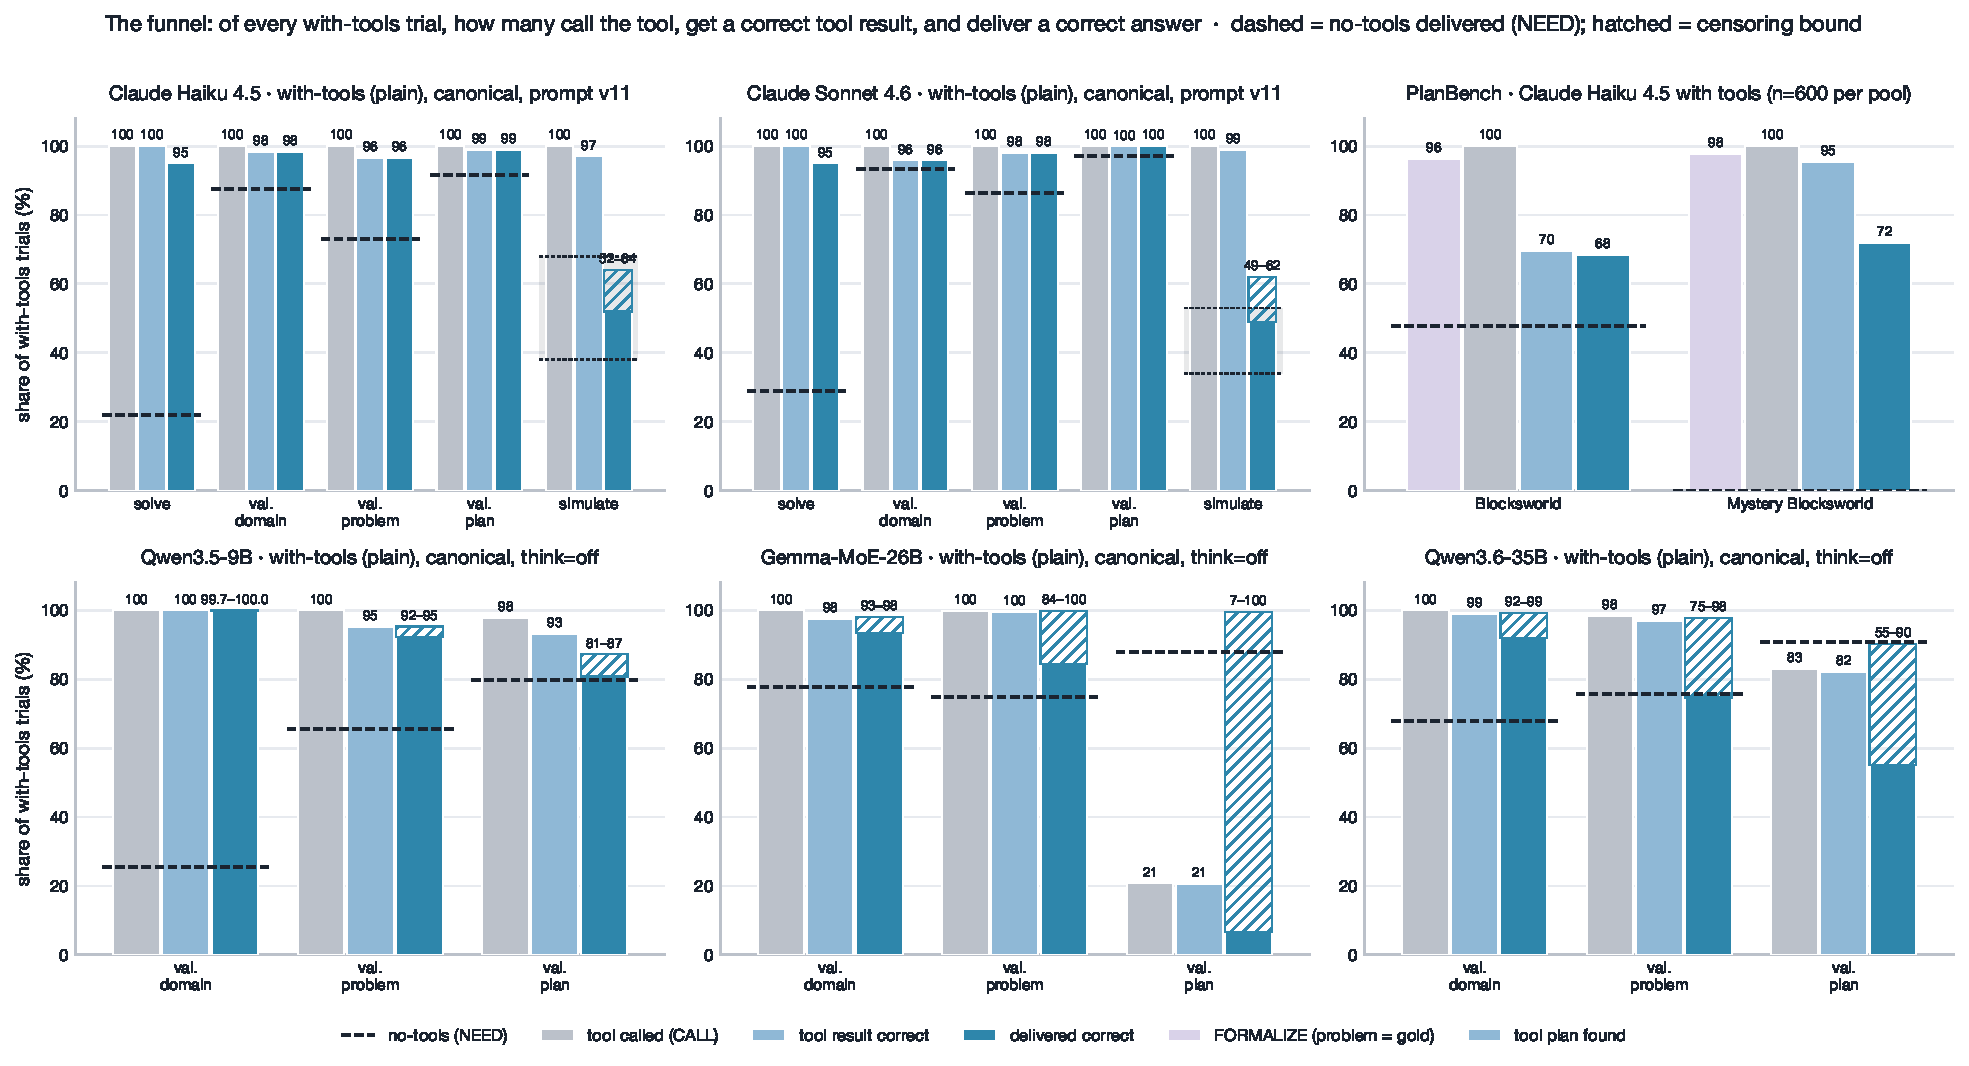
\includegraphics[width=\textwidth]{figures/funnel.pdf}
\caption{The funnel. For every with-tools trial, the share that calls the tool
(\textsc{call}), obtains a correct tool result (the mechanism layer), and
delivers a correct answer (the primary surface); the dashed line is the
no-tools delivered rate on the same task (\textsc{need}), drawn as a reference
and never as a bar, because arms are never pooled. Top row: the two frontier
tiers on the canonical corpus (prompt v11) and the PlanBench arm, whose
sequence gains a leading \textsc{formalize} stage (the model's PDDL matches the
gold problem) because the prompt supplies no PDDL there. Bottom row: the three
$\geq$9B open-weight models on the validation tasks, plain arm,
\emph{think}=off; this corpus's \emph{solve} and \emph{simulate} tool cells are
censoring bounds too wide to draw and are reported in Figure~\ref{fig:solesource}
and the text. Bars are marginal shares of all trials, not nested conditionals;
hatched segments are censoring bounds \cbnd{a}{b}; the PlanBench delivered bars
use the first-draw counts ($410/600$ and $431/600$).}
\label{fig:funnel}
\end{figure*}

We organize the evaluation around six research questions. The first four ask,
per task, whether and how the tool helps; the last two ask whether its advantage
tracks two difficulty axes:
\begin{enumerate}
\item[\textbf{RQ1.}] On the two file-validation tasks (\emph{validate\_domain},
\emph{validate\_problem}), where the unaided model has some competence, does tool
availability add value?
\item[\textbf{RQ2.}] On \emph{solve}, can the unaided model find valid plans, and how
much does the tool add?
\item[\textbf{RQ3.}] On \emph{validate\_plan}, a task the unaided model already does
well, does mere availability help or hurt, and does steering change the answer?
\item[\textbf{RQ4.}] On \emph{simulate}, can the unaided model produce an exact state
trajectory at all?
\item[\textbf{RQ5.}] Does the tool's advantage grow with plan length?
\item[\textbf{RQ6.}] Does it grow with object count?
\end{enumerate}

Two regime vocabularies appear below and should not be conflated. A \emph{task} axis
sorts the five tasks by their unaided baseline: \emph{sole-source} (no unaided
success), \emph{headroom} (a weak but improvable baseline), and \emph{mixed}
(availability can hurt). A separate \emph{cross-mode} axis (Robustness) sorts tasks
by whether the realizable benefit survives reasoning mode: \emph{robust},
\emph{budget-dependent}, and again \emph{sole-source}. The two axes share only the
word sole-source (a task with no baseline is sole-source either way) and are
otherwise independent. Table~\ref{tab:scorecard} is the task-axis scorecard: two
tasks (\emph{solve}, \emph{simulate}) essentially do not happen \emph{unaided}
under the deployed budget and format constraints;
two (\emph{validate\_domain}, \emph{validate\_problem}) are improved over weak
baselines; and one (\emph{validate\_plan}) is a two-layer case. There, at the
mechanism layer, mere availability collapses invocation for two of three
$\geq$9B models and a one-sentence nudge repairs it; at the delivered surface
the canonical corpus is censored into bounds that cannot decide the harm, and
the full-storage rerun shows that the model that stops \emph{calling} often
still \emph{answers} correctly, so the two layers genuinely disagree.

\begin{table*}[t]
\centering
\footnotesize
\begin{tabular}{@{}ll p{0.60\textwidth}@{}}
\toprule
\textbf{RQ / task} & \textbf{verdict} & \textbf{evidence ($\geq$9B, \emph{think}=off)} \\
\midrule
RQ1 \emph{validate\_domain} / \emph{validate\_problem} & \textsc{yes} &
\emph{validate\_domain}: delivered lower bounds $92$--$100\%$ with the tool
against exact unaided $26$--$78\%$; favorable for all three even if every
censored trial failed. \emph{validate\_problem}: favorable for the 9B
($\geq$$92.2$ vs $65.7$); Gemma favorable at 95\% but not after the clustering
correction; the 35B cell straddles and stays undecided; none against \\
RQ2 \emph{solve} & \textsc{yes} & unaided floored at $8$--$11\%$ (exact); at the
frontier tier the lift is exact and delivered: $22\!\to\!95\%$ (Haiku),
$29\!\to\!95\%$ (Sonnet). Open-roster tool cells are bounds: the 9B survives the
worst case (\cbnd{26.0}{58.7} vs $10.7$), a margin under $1$\,pp after the
clustering correction, so we read it as exploratory; Gemma and the 35B are
undecided \\
RQ3 \emph{validate\_plan} & \textsc{undecided} (delivered); \textsc{mixed}
(mechanism) & at the mechanism layer availability collapses Gemma's invocation
to $21\%$ of trials ($-67$\,pp tool-verified) and steering repairs it; on the
delivered surface all three canonical cells are censored into straddling bounds,
and the full-storage rerun \emph{inverts} the Gemma cell: delivered
\cbnd{30.0}{63.1} against tool-verified $0.9\%$ \\
RQ4 \emph{simulate} & \textsc{no} as deployed & unaided: $0\%$ format-exact on
the shared-budget corpus; $22$--$40\%$ content-correct once budgets are
decoupled, and \cbnd{41.7}{61.3} at the frontier. With tools, delivered is
undecided on the canonical corpus and \cbnd{49}{62}/\cbnd{52}{64} at the
frontier, not separated from the frontier unaided cell; the mechanism layer runs
at $97$--$99\%$, and that delivery gap is the finding \\
RQ5 plan length & \textsc{yes} (mechanism layer) & \emph{validate\_plan}
advantage widens $+5\!\to\!+7\!\to\!+27$\,pp with reference length \\
RQ6 object count & \textsc{no} (mechanism layer) & \emph{validate\_problem}
advantage flat ($+22/{+}23/{+}23$\,pp) across object-count bins \\
\bottomrule
\end{tabular}
\caption{Scorecard: six research questions on the delivered surface. A gap
counts as favorable evidence only if the two arms' 95\% intervals are disjoint
\emph{and} it points the hypothesized way; disjoint gaps pointing the other way
are tallied as significant-against (Methodology). Cells written \cbnd{a}{b} are
censoring bounds and support a verdict only at their claim-adverse end; rows
marked mechanism layer are computed on tool-verified rates, which are exact in
every corpus, and are labeled because they measure the tool path rather than the
delivered answer.}
\label{tab:scorecard}
\end{table*}

\begin{figure*}[t]
\centering
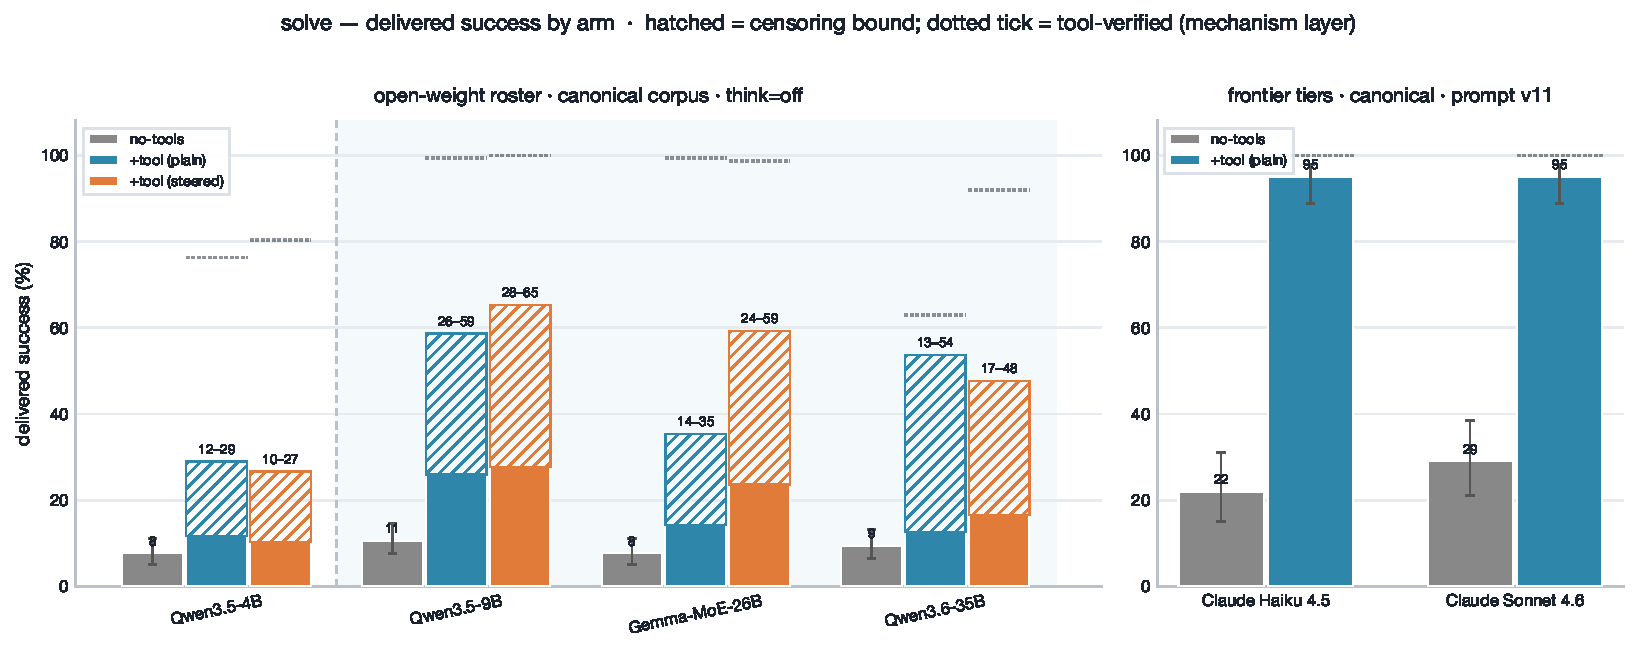
\includegraphics[width=0.49\textwidth]{figures/solve.pdf}\hfill
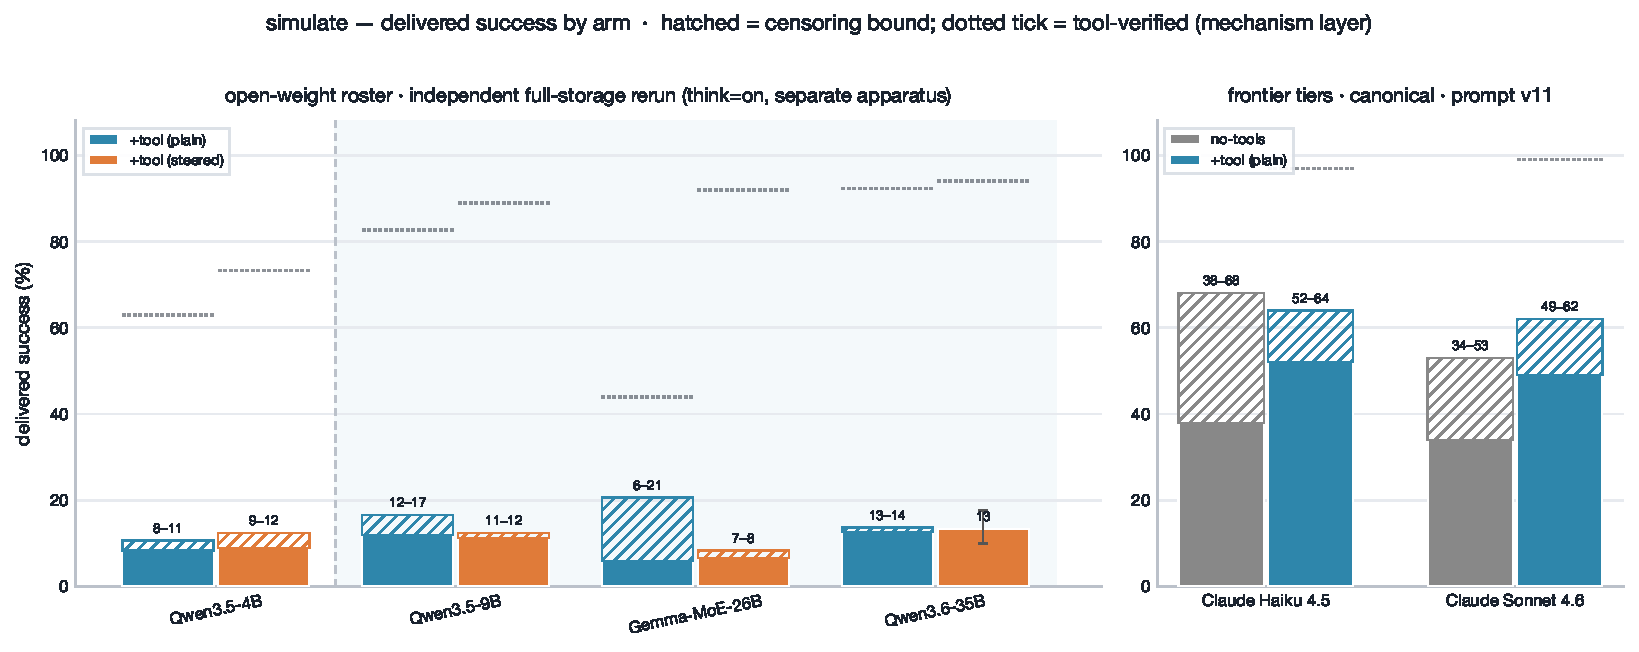
\includegraphics[width=0.49\textwidth]{figures/simulate.pdf}
\caption{Sole-source tasks on the delivered surface (\emph{think}=off). Solid
bars are delivered rates, hatched segments are censoring bounds \cbnd{a}{b},
whiskers are Wilson 95\% intervals on exact cells, and the dotted tick above a
tool bar marks the mechanism layer (tool-verified). \emph{solve} (left): the
open-weight roster on the canonical corpus (the $\geq$9B headline set is
shaded) and the two frontier tiers (prompt v11, exact). Unaided \emph{solve} is
floored at $8$--$11\%$ open-weight and $22$--$29\%$ at the frontier; with the
tool the frontier delivers $95.0\%$ at both tiers against a $100\%$ mechanism
layer, while the open-weight tool arms clear their baselines only at the
claim-adverse end of the 9B's bound. \emph{simulate} (right): the canonical
open-weight cells are censored on both arms, so the open-weight panel shows the
independent full-storage rerun (\emph{think}=on, separate apparatus,
within-corpus contrasts only), where the tool verifies $44$--$94\%$ of
trajectories per cell but at most \cbnd{6}{21} is delivered; the frontier panel
shows delivered \cbnd{49}{62} (Sonnet) and \cbnd{52}{64} (Haiku) against
unaided \cbnd{34}{53} and \cbnd{38}{68}, which the bounds do not separate.}
\label{fig:solesource}
\end{figure*}

\subsection{Two Tasks the Model Cannot Do Unaided}
\emph{Solve} and \emph{simulate} are sole-source on the baseline side: unaided,
they essentially do not happen (Figure~\ref{fig:solesource}). Unaided
\emph{solve} is floored at $8$--$11\%$ across the $\geq$9B models, exactly
measured. What the tool delivers back is cleanest at the frontier tier, where
storage permits exact delivered rates: Claude Haiku 4.5 rises
$22\!\to\!95\%$ and Claude Sonnet 4.6 $29\!\to\!95\%$, both CI-disjoint, both
sitting exactly $5.0$\,pp under their own mechanism layer of $100\%$ (the
delivery-gap analysis below takes up those five points). On the open-weight
roster the tool arm's delivered rates are censoring bounds: the 9B's
\cbnd{26.0}{58.7} clears its $10.7\%$ baseline even if every censored trial
failed, though by under a point once the clustering correction is applied, so we
read it as exploratory; Gemma (\cbnd{14.3}{35.3}) and the 35B
(\cbnd{12.7}{53.7}) straddle and stay undecided (RQ2 \textsc{yes}, carried by
the frontier tier and the baseline floor). The mechanism layer says why the
open-roster bounds sit so far under their tool-verified rates of $63$--$99\%$:
invocation. Where the plain arm leaves headroom (Qwen3.6-35B invokes the
planner on only $68\%$ of trials) steering raises invocation
to $94\%$, and every $\geq$9B model is $\geq$93\%
accurate when it does call the planner, so what limits the tool path on
\emph{solve} is invocation frequency.

\emph{Simulate} is more extreme: unaided \emph{format-exact} success is $0\%$ for
every open-weight model, in both
reasoning modes, across all $3{,}000$ trials (a rule-of-three $95\%$ upper bound of
$\leq$0.1\%). The tool runs the simulation correctly at the mechanism layer on
$65$--$92\%$ of plain-arm trials ($83$--$97\%$ steered), but almost none of that
reaches the delivered answer on this corpus: not one open-roster tool-arm trial
yields a determinate delivered success, and the bounds top out at
\cbnd{0}{20}--\cbnd{0}{39} for the $\geq$9B models. The determinate failure mass
is dominated by trials in which the model drives the tool correctly and then
exhausts its decode budget before restating the trajectory, a with-tools failure
mode in its own right. The unaided zero, meanwhile, is a property of the deployed budget
and format constraints, not an absent capability. Success demands
canonical-form deep-equality of the \emph{entire} state trajectory against the
oracle (structured JSON, no partial credit, no free-text fallback), and the
unaided failures decompose ($\geq$9B) into $68\%$ unparseable trajectory JSON,
$29\%$ truncated at the $6{,}144$-token cap, and only $3\%$ parsed-but-wrong
(Figure~\ref{fig:failtax}): the models fail on format and budget before content is
tested. A budget-decoupled control isolates the content question. Giving the
reasoning trace and the answer separate decode allowances (a two-call continuation
that stops decoding at the think-close tag; \emph{think}=on, Qwen roster, run as a
separate corpus never pooled with the main one) and grading with a wrapper-tolerant
two-metric grader, unaided content-correct state tracking rises to $23.0\%$ (4B),
$22.3\%$ (9B), and $40.0\%$ (35B), with the $0.8$B model alone still at $0\%$;
re-grading the main corpus's stored responses under the same tolerant grader
recovers at most $0.7\%$, so the recovery comes from the budget, not the grader.
Format compliance stays $0\%$ for all four models (none ever emits the exact
requested wrapper), so strict content-and-format success remains $0\%$ across the
board. The honest comparison in the matching mode is therefore
$22$--$40\%$ content-correct unaided against a tool-arm mechanism layer of
$87$--$96\%$; a delivered-surface version of that contrast cannot be computed
from this corpus (the tool arm delivers no determinate trajectory), and the
claim ``these models cannot track state at all'' does not
survive the control.

\begin{figure*}[t]
\centering
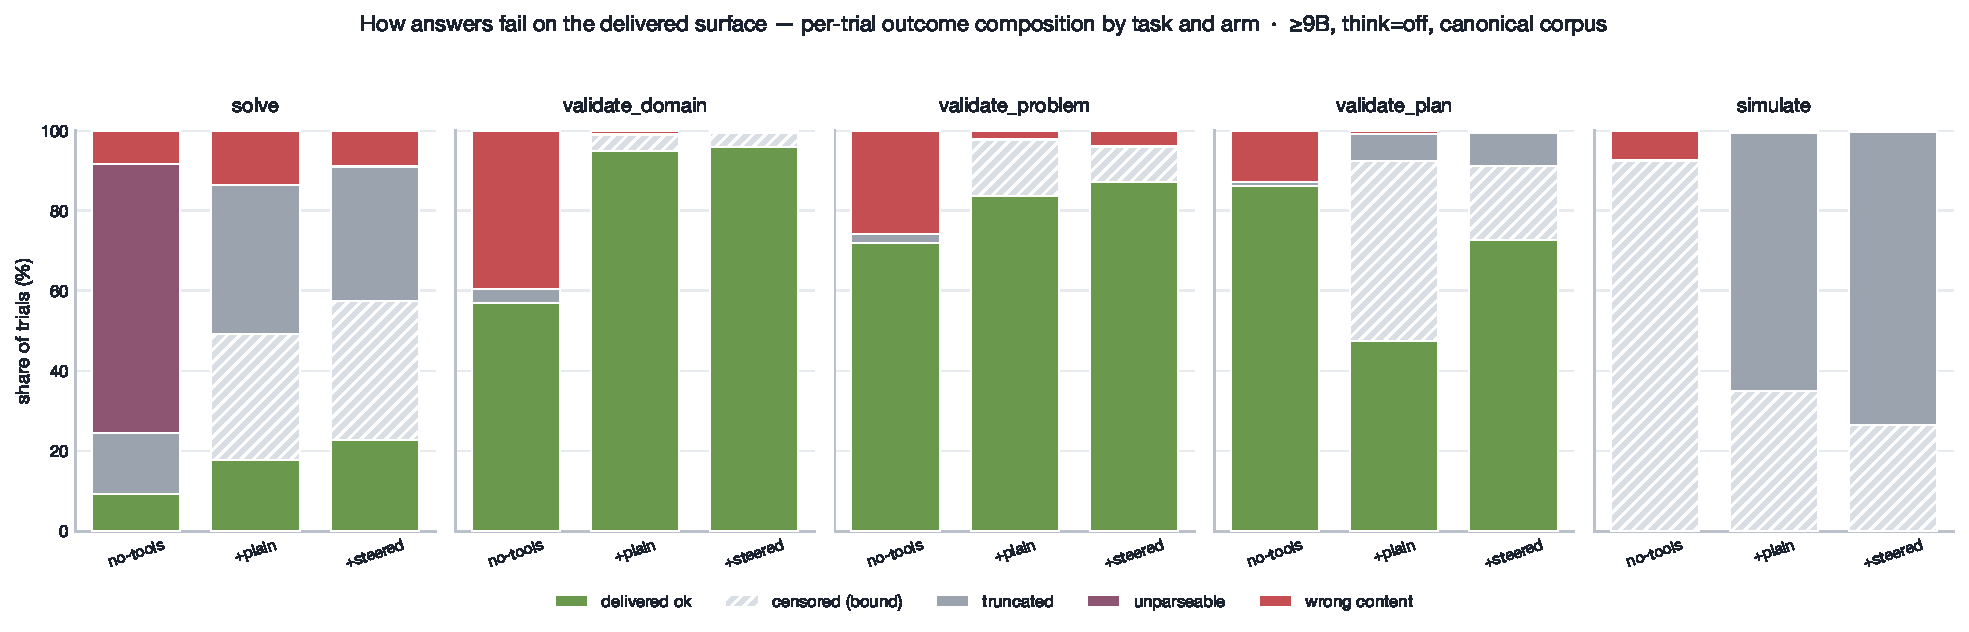
\includegraphics[width=\textwidth]{figures/failure_taxonomy.pdf}
\caption{How answers fail on the delivered surface: per-trial outcome
composition by task and arm ($\geq$9B, \emph{think}=off, canonical corpus,
pooled), each bar normalized to $100\%$. Every trial is \emph{delivered ok} or
exactly one other outcome: \emph{censored} (the stored snapshot ends before the
answer can be graded, a bound rather than a failure), \emph{truncated} (the
budget ran out with no answer), \emph{unparseable}, or \emph{wrong content}.
Unaided \emph{solve} is $67\%$ unparseable and $15\%$ truncated; the unaided
validation baselines fail by wrong content ($13$--$40\%$); on the tool arms the
dominant non-success mass is censoring, which is why those cells are bounds, and
on \emph{validate\_plan} the plain arm's censored band is largely the trials in
which the model reasons in prose instead of calling the validator, the silence
that steering removes (Figure~\ref{fig:mechanism} shows it at the mechanism
layer). Unaided \emph{simulate} on this corpus is $93\%$ censored under the
delivered grader; its online-grader anatomy ($68\%$ unparseable, $29\%$
truncated) is quoted in the text.}
\label{fig:failtax}
\end{figure*}

\subsection{The Delivery Gap: What Reaches the Answer}
The two grading layers let us measure something the tool-use literature usually
cannot see: how much of what the tool computes actually reaches the model's
answer. Table~\ref{tab:deliverygap} (and the top row of Figure~\ref{fig:funnel})
reports both layers for the frontier
with-tools runs, where storage permits exact delivered rates. The pattern is
sharp and identical at both capability tiers. On the three validation tasks the
gap is zero to within a tenth of a point: a verdict is a short string, and the
model that obtains it restates it. On \emph{solve} both models deliver $95.0\%$
against a mechanism layer of $100\%$: a $+5.0$\,pp gap with the same failure
anatomy at both tiers. Every Sonnet failure is a transcription error made while
restating the tool-validated plan into the final answer (five plans, zero
omissions); Haiku's five are three transcription errors and two omissions. On
\emph{simulate} the gap opens to tens of points: the tool runs the trajectory
correctly on $97$--$99\%$ of trials, and the delivered rate is
\cbnd{52}{64} (Haiku) and \cbnd{49}{62} (Sonnet). Half the Sonnet failure mass
is output budget (trajectories cut mid-stream or censored at the cap), the rest
split between answers with no coercible trajectory and wrong state content.

The gap therefore tracks the length of what must be restated: a verdict (words)
loses nothing, a plan (lines) loses five points, a trajectory (full state dumps)
loses a third or more. A stronger model does not close it: Sonnet and Haiku tie
at $95.0$ on \emph{solve} with the same five-failure count, and their
\emph{simulate} bounds overlap almost completely. On this evidence the gap is a
property of answer length interacting with the output budget, not of model
strength.

The open-weight roster shows the same structure wherever it can be measured. On
the canonical corpus the tool arms' delivered rates are bounds, so the gap is
bounded rather than pointed; the full-storage rerun (Table~\ref{tab:howtoread};
within-corpus contrasts only) makes it exact for open models: \emph{simulate}
delivered reaches only \cbnd{8.3}{10.7} (4B), \cbnd{12.0}{16.7} (9B), and
\cbnd{12.7}{13.7} (35B) against mechanism layers of $63$, $83$, and $92\%$. The
same corpus also shows the gap can run \emph{backwards}: on Gemma's
\emph{validate\_plan} cell the mechanism layer is $0.9\%$ (the model almost
never completes a valid tool interaction) while the delivered rate is
\cbnd{30.0}{63.1}, because the model answers the verdict question directly, in
prose, without the tool. Not calling is not the same as not answering, a point
the availability analysis below has to respect.

\begin{table}[t]
\centering
\small
\begin{tabular}{@{}lcc@{\hspace{1.2em}}cc@{}}
\toprule
& \multicolumn{2}{c}{\textbf{Haiku 4.5}} & \multicolumn{2}{c}{\textbf{Sonnet 4.6}} \\
\textbf{Task} & \textbf{deliv.} & \textbf{mech.} & \textbf{deliv.} & \textbf{mech.} \\
\midrule
\emph{validate\_domain}  & $98.3$ & $98.3$ & $95.8$ & $95.8$ \\
\emph{validate\_problem} & $96.5$ & $96.5$ & $98.0$ & $98.0$ \\
\emph{validate\_plan}    & $98.8$ & $98.9$ & $100.0$ & $99.9$ \\
\emph{solve}             & $95.0$ & $100.0$ & $95.0$ & $100.0$ \\
\emph{simulate}          & \cbnd{52}{64} & $97.0$ & \cbnd{49}{62} & $99.0$ \\
\bottomrule
\end{tabular}
\caption{The delivery gap at the frontier: delivered success against the
mechanism layer (tool-verified), with-tools plain arm, canonical corpus,
\emph{think}=off equivalent. $n$ per task: $120$ / $200$ / $1{,}000$ / $100$ /
$100$. Delivered \emph{simulate} cells are censoring bounds ($12$--$13$ of
$100$ trials censored at the $16$K snapshot); every other cell is exact (Wilson
95\% intervals in the text). The gap is $\approx$0 on verdict-length answers,
$+5.0$\,pp on plans at both tiers, and $\geq$33\,pp on trajectories.}
\label{tab:deliverygap}
\end{table}

\subsection{Two Validation Tasks: Headroom and Rescue}
On \emph{validate\_problem} the unaided model is genuinely partly competent: the set
is balanced one-to-one, so a constant ``VALID'' guess scores $\approx$50\%, and the
$\geq$9B models clear that floor before any tool ($65.7$--$75.7\%$, exact). On the
delivered surface the availability picture is favorable where it can be decided
and undecided where it cannot: the 9B rises to \cbnd{92.2}{95.3}, clearing its
baseline even if every censored trial failed; Gemma's \cbnd{84.3}{99.8} clears at
the 95\% level but by too little to survive the paraphrase-clustering correction,
so we flag it as near-threshold; and the 35B's \cbnd{74.7}{97.8} straddles its
$75.7\%$ baseline and stays undecided. No model moves against (RQ1 \textsc{yes},
qualified). \emph{Validate\_domain} behaves
differently. Because its fixtures run $5{:}1$ valid-to-invalid, a constant
``VALID'' already scores $83\%$; yet unaided, every $\geq$9B model lands \emph{at or
below} that trivial line (pooled $26$--$78\%$) and discrimination is unreliable across
the board, from near-chance to only modest (balanced accuracy $53$--$74\%$; Table~\ref{tab:vdom}). Qwen3.5-9B is the clearest
case: it answers
``INVALID'' almost reflexively (true-positive rate $12\%$, true-negative rate
$95\%$), scoring $26\%$ pooled but $53\%$ balanced. The tool does not \emph{refine} a
competent baseline here; it \emph{rescues} a task the models cannot do reliably.
The delivered lower bounds alone establish it: \cbnd{99.7}{100.0} (9B),
\cbnd{93.3}{98.1} (Gemma), and \cbnd{91.9}{99.2} (35B) against exact unaided
baselines of $26$, $78$, and $68\%$, favorable for all three at the claim-adverse
end and past the $83\%$ trivial line at every lower bound. Balanced accuracy on
the delivered surface tells the same story: the steered arm reaches
\cbnd{100}{100} (9B), \cbnd{92.2}{95.0} (Gemma), and \cbnd{82.7}{99.2} (35B)
against unaided $53$, $74$, and $65\%$, clearing the baseline at the
claim-adverse end for all three; the 35B's wide bound comes from its
$60$-trial negative arm, of which $19$ are censored (Table~\ref{tab:vdom}). The
\emph{validate\_domain}
verdict holds from 4B up (\cbnd{84.2}{100.0} against $19.2\%$); the 4B's
\emph{validate\_problem} cell is undecided. The 0.8B model moves sharply and
decidedly \emph{against} on both tasks even at the censoring bounds' favorable
end (\emph{validate\_domain} $80.8\!\to\!$\cbnd{43.9}{45.8};
\emph{validate\_problem} $51.2\!\to\!$\cbnd{4.0}{5.8}): small-model
tool-mishandling, in which it calls the right tool but omits required arguments,
costs it answers it could have produced unaided. Steering
does not help either validation task at the mechanism layer
($-5$--${+}1$\,pp); the one
CI-disjoint movement (a $-5$\,pp dip on \emph{validate\_problem} for the 9B)
points mildly against and does not survive the paraphrase-clustering correction
above, so we treat it as non-confirmatory. Once a capable model has the tool it
already calls it, and the nudge matters only where the plain arm under-calls, as in
the next case.

\begin{figure}[t]
\centering
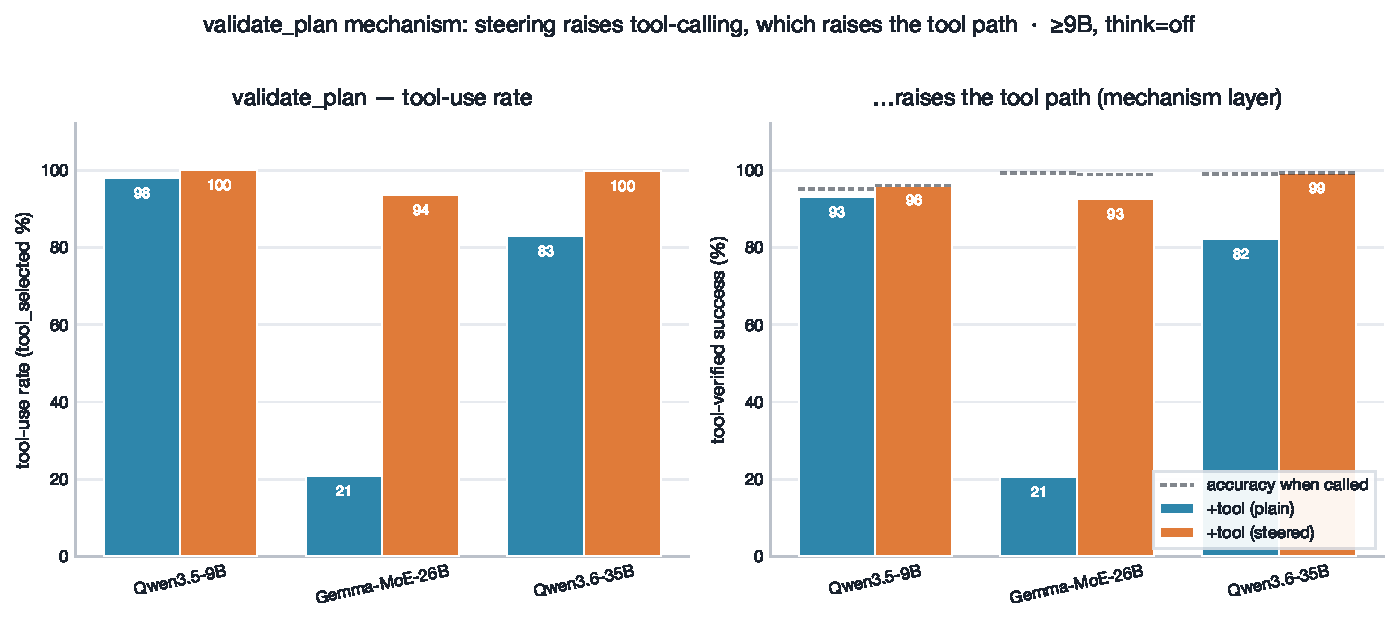
\includegraphics[width=\columnwidth]{figures/mechanism_validate_plan.pdf}
\caption{\emph{validate\_plan} mechanism ($\geq$9B, \emph{think}=off). Left:
tool-use rate (plain vs.\ steered); right: mechanism-layer (tool-verified)
success. Where the plain arm under-calls
the validator (Gemma-MoE), steering restores invocation, and the tool path rises
with it: the tool's value is gated on the model actually calling it. Both panels
are exact in every corpus (tool transcripts are stored in full).}
\label{fig:mechanism}
\end{figure}

\subsection{When Availability Backfires at the Tool Path, and Steering Repairs It}
\emph{Validate\_plan} is the one task the unaided model already does well
($\geq$9B no-tools $80$--$91\%$, exact), and it is where the two grading layers
tell visibly different stories, so we give both and keep them labeled.

At the mechanism layer the picture is dramatic and exact. Merely making the
tool available collapses the tool path for two of three $\geq$9B models:
Gemma-MoE-26B's tool-verified rate falls $88\!\to\!21\%$ ($-67$\,pp) and
Qwen3.6-35B's $91\!\to\!82\%$ ($-9$\,pp); only Qwen3.5-9B improves
($80\!\to\!93\%$, $+13$\,pp). The decomposition pins the cause. Writing
tool-path success as $P(\text{call})\times P(\text{correct}\mid\text{call})$,
Gemma's collapse is entirely in the first factor: under the plain prompt it
calls the validator on only $21\%$ of trials, but \emph{when it calls it is
$99\%$ correct}. Steering moves only $P(\text{call})$ (from $21\!\to\!94\%$) and
the mechanism layer follows it almost exactly ($0.94\times0.99=0.93$;
Figure~\ref{fig:mechanism}). Across every $\geq$9B tool
cell except 9B \emph{simulate} ($\approx$81\%), $P(\text{correct}\mid\text{call})$
stays $\geq$92\% and varies little between arms (Table~\ref{tab:decomp}); nearly
all between-arm and between-model variance
at this layer is variance in \emph{whether the model calls}. These rates are
computed from the stored tool transcripts and are exact in every corpus.

On the delivered surface, the canonical corpus cannot decide whether that
collapse hurt the user's answer. All three $\geq$9B tool cells are censored into
straddling bounds (Gemma \cbnd{6.6}{99.6} with $93\%$ of snapshots censored; the
35B \cbnd{55.0}{90.3} against $90.9$; the 9B \cbnd{80.8}{87.2} against $79.7$),
so the availability gap on this task is \emph{undecided} at the primary surface,
in both directions: neither the $-67$\,pp harm nor the $+13$\,pp lift survives as
a delivered claim here. The full-storage rerun says why caution is warranted:
in that corpus Gemma's delivered rate is \cbnd{30.0}{63.1} while its mechanism
layer is $0.9\%$. The model that almost never completes a tool call still
answers the verdict question directly, in prose, and is often right. Not
calling is not the same as not answering, so a collapse of the tool path only
bounds, and does not determine, the collapse of the answer. What survives at
full strength is the invocation finding itself: availability swings whether the
model uses the tool by huge, model-specific amounts, and one directive sentence
moves invocation from $21\%$ to $94\%$.

This also explains an apparent size inversion. In the plain arm's mechanism
layer the 9B
``beats'' the 35B (\emph{solve} $99\%$ vs.\ $63\%$; \emph{validate\_plan} $93\%$
vs.\ $82\%$), but this reflects tool-call \emph{propensity}, not capability: the
tool path tracks tool-use almost 1:1, accuracy-given-a-call is $\geq$93\% for both, and
steering closes the gap (35B \emph{solve} $63\!\to\!92\%$ at that layer). The propensity even
flips with reasoning mode (under \emph{think}=on the 35B calls the validator on
$99.9\%$ of trials, the 9B on $69\%$). The 35B's unaided baselines exceed the 9B's
on every validation task; the inversion is a behavioral difference in spontaneous
tool adoption rather than a capability gap. Because our two largest models are AWQ-INT4
while the 9B is 16-bit, we read this cross-model inversion as a propensity
phenomenon we observe rather than a controlled size effect (see Limitations).

\subsection{Does the Advantage Track Difficulty?}
These two difficulty analyses run at the mechanism layer (the tool-arm side of
each bin contrast is tool-verified, since binned delivered rates on the
canonical corpus are bounds too wide to compare), and are labeled accordingly.
An advantage can only be \emph{seen} to change where the no-tools baseline has room
to move, which makes \emph{validate\_plan} the case where this is visible (RQ5 \textsc{yes}):
as the reference plan lengthens, unaided accuracy degrades
($94\!\to\!91\!\to\!62\%$ over short/medium/long bins) while the tool path holds
($\approx99\!\to\!98\!\to\!89\%$), so the gap widens $+5\!\to\!+7\!\to\!+27$\,pp;
the harder the instance, the more the tool is worth. The other two length-sensitive
tasks bracket this case: \emph{solve}'s gap is large but roughly constant
($+87\!\to\!+87\!\to\!+89$\,pp), both arms pinned (baseline floored, tool near
ceiling); \emph{simulate}'s gap is large but \emph{declines}
($+100\!\to\!+93\!\to\!+77$\,pp, CI-disjoint), because although its baseline stays
floored at $0$, the tool arm itself degrades on long trajectories, the one place
tool-assisted success erodes with difficulty. Object count, by contrast, moves
nothing: the \emph{validate\_problem} gap is flat at $+22/{+}23/{+}23$\,pp and the
other tasks are flat too (RQ6 \textsc{no}). Plan length is a difficulty axis the
tool's advantage tracks; object count is not.

\begin{figure*}[t]
\centering
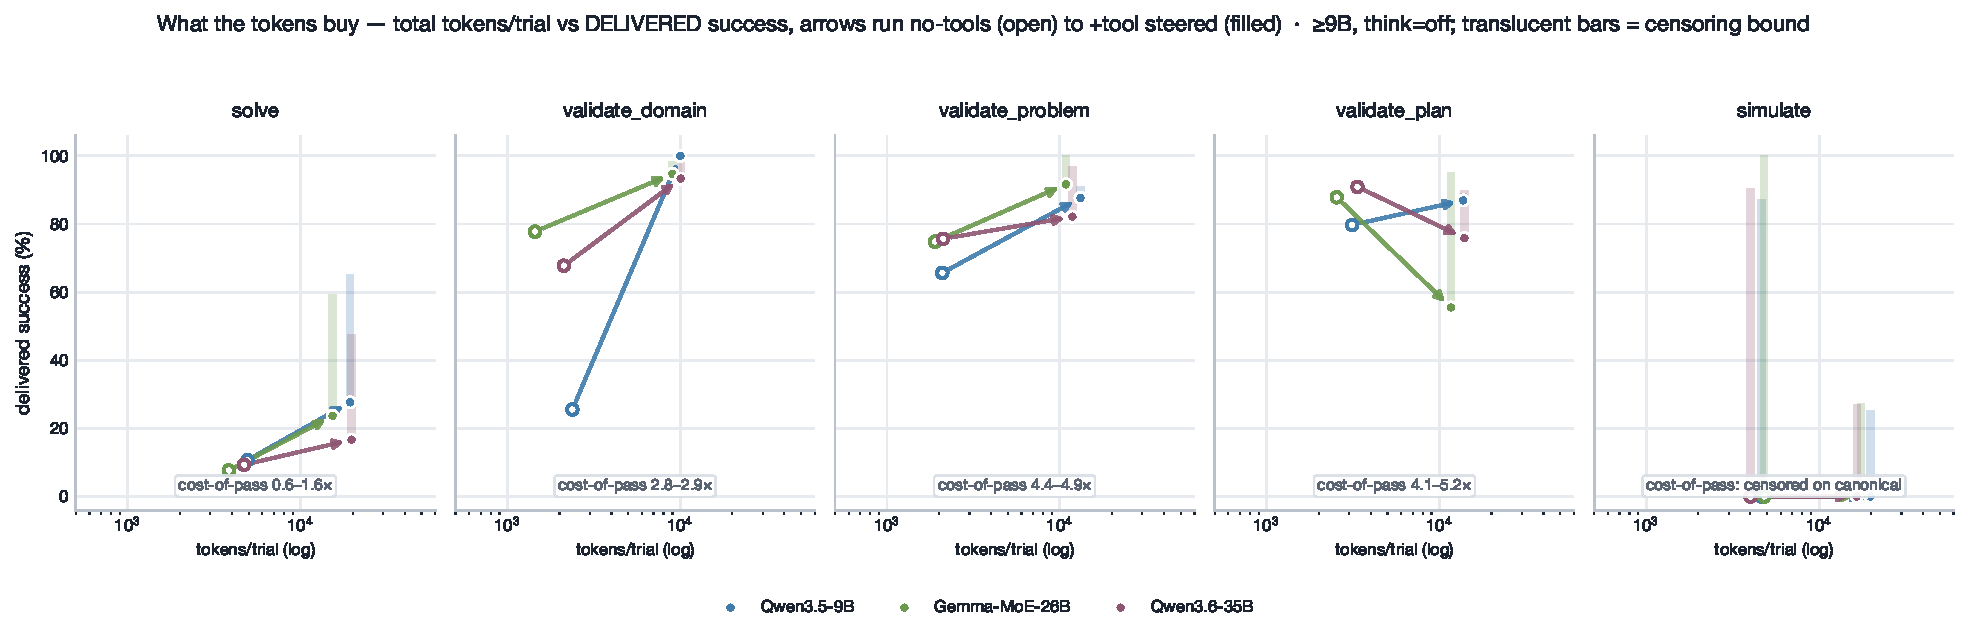
\includegraphics[width=\textwidth]{figures/token_quadrant.pdf}
\caption{What the tokens buy ($\geq$9B, \emph{think}=off): mean total tokens per
trial (log $x$) vs.\ delivered success ($y$); each arrow runs
no-tools$\to$+tool(steered), and a translucent bar marks a censoring bound.
Every arrow points right: the tool always costs more per trial. Delivered
cost-of-pass (tokens per delivered success, as a range across the bound) is
$0.6$--$1.6\times$ the unaided cost on \emph{solve}, $2.8$--$5.2\times$ on the
validation tasks, and not identified on \emph{simulate}, where both arms are
censored on this corpus.}
\label{fig:tokens}
\end{figure*}

\subsection{What the Tool Costs}
The tool is not free (Figure~\ref{fig:tokens}). Per trial it raises total token
consumption (input~$+$~output, summed over turns) several-fold:
$\approx$4--6$\times$ on the $\geq$9B models, and up to $\approx$15$\times$ for the
smaller 4B. The added cost is \emph{input} rather than output: the unaided model is
output-heavy (input:output $\leq$1:1, as low as $0.3$:1 on \emph{solve}, where it reasons in the open), while the
tool arms are strongly input-heavy ($\approx$6--12:1) because the tool schemas and tool outputs
are re-fed every turn. (Server-side prefix caching, $\approx$90\% on this roster,
makes the re-fed \emph{schemas} cheap to compute, but tool \emph{outputs} are
uncached and the tokens are still real context. Our token totals count these raw, so where
caching applies the tool's reported cost is, if anything, an over-estimate.) A
production system could lower the input overhead further by not re-feeding full tool
outputs on every turn, summarizing or eliding them once consumed; our harness re-feeds
them verbatim, so the cost-of-pass we report is a faithful worst case rather than a
deployment-tuned figure.

Whether it is worth paying depends entirely on the baseline: the choice of
metric flips the verdict by $\approx$10$\times$ on identical data, so we report
\emph{cost-of-pass} $=$ total tokens $\div$ successful trials (lower is better),
which factors exactly as (tokens-per-trial ratio) $\div$ (success-rate ratio).
On this corpus the tool arms' delivered rates are bounds, so these ratios count
successes at the mechanism layer and are labeled tool-path economics; a
delivered-surface cost-of-pass can only be equal or costlier, since delivered
successes are a subset of tool-verified ones.
Where the baseline is floored the tool pays for itself: on \emph{solve} it is
$\approx$0.3--0.4$\times$ the cost per success (e.g.\ $\approx$4$\times$ more tokens
$\div$ $\approx$9--13$\times$ more correct answers); on the delivered surface the
same ratio is a range, $0.6$--$1.6\times$, because the tool arm's delivered
successes are bounded (Figure~\ref{fig:tokens}). At the frontier, where
delivered \emph{solve} is exact, the verdict inverts: the unaided baseline is no
longer floored ($22$--$29\%$) and the re-fed context dominates, so a delivered
pass costs $3.1\times$ (Sonnet, $18.6$K vs.\ $6.0$K tokens) and $6.1\times$
(Haiku, $48.5$K vs.\ $8.0$K) the unaided tokens, and on \emph{simulate}
\cbnd{84}{106}K against \cbnd{10}{15}K (Sonnet), a $5$--$11\times$ premium
per delivered trajectory. On \emph{simulate} the
unaided arm produces no format-exact success here, but the tool arm also rarely
delivers its trajectory within budget, so at the delivered level neither arm's
per-success cost is identified on this corpus and we make no \emph{simulate}
cost claim beyond the mechanism layer. Where
the baseline is already strong the tool is a luxury: $\approx$3--5$\times$ costlier
per success on most \emph{validate\_*} cells ($\geq$9B), where it is only modestly
more often right and the token premium dominates. The picture is therefore mixed:
\emph{the tool is cost-effective where the model cannot do the task without it}, and
a token-priced luxury where it can. Because cost-of-pass is a
token \emph{ratio}, it is invariant to the per-token price: at representative commodity serving
rates (order \$0.1--\$1 per million tokens) the absolute cost is a fraction of a cent per correct
answer on the floored tasks, but the comparative verdict does not turn on that rate. We report token
cost rather than wall-clock latency because the batched server multiplexes trials, so per-trial
latency is not recoverable from our logs; a concurrency-one benchmark is the right future
instrument for the time axis. (The output
cap right-censors long generations; raw ``hit-cap'' rates are not comparable across
arms, since tool runs are multi-turn: a cap-hit
on a final narration turn does not void the tool's verified result, so
cap-hit-and-failed stays
$\leq$10\% in the tool arms at the mechanism layer, though the same cap-hit can
censor or fail the delivered answer. We report totals; a completion-only view, which
makes the tool look better, we do not report.)

\subsection{Robustness: Reasoning Mode and Contamination}
\textbf{Reasoning mode.} At the mechanism layer, the same signed rule applied to
the \emph{think}=on
corpus reproduces the verdict pattern (\textsc{yes}/\textsc{yes}/\textsc{mixed}/%
\textsc{yes}, RQ5 \textsc{yes}, RQ6 \textsc{no}); the delivered surface under
\emph{think}=on carries the same censoring bounds as at \emph{think}=off and adds
no decided cell. But the raw \emph{think}=on
gaps are budget-confounded: reasoning and answer share one decode budget
($6{,}144$ tokens; $8{,}192$ for \emph{solve}), and $14$--$92\%$ of $\geq$9B
no-tools \emph{think}=on trials truncate (Gemma-MoE-26B $92\%$, the 35B only $14\%$), collapsing the validation baselines
(\emph{validate\_plan}: 9B $80\!\to\!21\%$, Gemma $88\!\to\!10\%$;
\emph{validate\_domain} Gemma $78\!\to\!0\%$). We therefore read the cross-mode
evidence only through budget-insensitive statistics. The steered tool arm is
mode-stable at the mechanism layer (mean off-vs-on shift $9$\,pp; the 35B is
invariant on all five tasks)
while the no-tools baseline swings $28$\,pp, so nearly all cross-mode movement
is a baseline effect rather than a change in the tool's value. The robust floor (the
minimum benefit over both modes, computed at the mechanism layer) keeps
\emph{solve} robust ($+46$--$71$\,pp) and
\emph{simulate} sole-source ($+83$--$97$\,pp; a benefit with no baseline cannot be
budget-confounded); the \emph{validate\_*} tasks are budget-dependent, their large
\emph{think}=on gaps being the artifact.

\textbf{Contamination.} Because the domains are public, we re-ran the matrix on
structurally identical domains with all surface names renamed
(Table~\ref{tab:contam}). The \emph{think}=off no-tools probe is near-null (mean
$|\Delta(\mathrm{canonical}-\mathrm{anonymized})|$ success $1.1$\,pp, max $3.7$, with
zero CI-disjoint task cells), so the unaided baseline carries no detectable
memorization signal where it has headroom, and the availability gaps are not a
contamination artifact. The per-task breakdown (Table~\ref{tab:contam-pertask})
sharpens this: across the $15$ $\geq$9B (model\,$\times$\,task) cells the mean
$|\Delta|$ is $1.2$\,pp (max $3.7$), confirming the null task-by-task, and the
largest drifts all favor the \emph{anonymized} corpus, the opposite of the
direction memorization of the public domains would produce. The only CI-disjoint cell anywhere is \emph{validate\_plan}
under \emph{think}=on, and it traces to tokenization rather than memory: the renamed
prompts run $\approx$5\% longer and so truncate more under the shared budget, so
success falls $4$--$6$\,pp in lockstep with completion while success-given-completion
is unchanged. This is itself a demonstration of the budget confound above.

\textbf{A budget-decoupled control.} Because the shared decode budget confounds the
\emph{think}=on unaided baseline, we re-ran the unaided arm under the decoupled
apparatus described in the \emph{simulate} results (separate reasoning and answer
allowances; Qwen roster; a separate corpus, never pooled with the main sweep).
Beyond the \emph{simulate} recovery reported there ($22$--$40\%$ content-correct at
$\geq$4B), validation baselines rise sharply (e.g.\ \emph{validate\_plan}
$+34$--$60$\,pp for 4B/9B, Wilson-disjoint), while \emph{solve} is flat for 9B/35B
and drops $6$\,pp at 4B, so decoupling is not uniformly beneficial. The tool
verdicts are unchanged; what shrinks is the unaided floor, to its honest size.

\textbf{A frontier proprietary model.} To test whether these baseline properties
hold beyond the open-weight roster, we re-ran the no-tools arm on Claude Sonnet 4.6,
a strong proprietary model, over both corpora at full $N$ (\emph{think}=off;
Table~\ref{tab:frontier}). The \emph{solve} floor carries over: unaided success is
$28.7\%$, above the open roster's $8$--$11\%$, so the frontier model retains modest
unaided planning ability but still fails on more than two thirds of problems without
the tool. The \emph{simulate} floor does not carry over: after de-censoring from the raw
batch output, Sonnet's unaided canonical cell is \cbnd{41.7}{61.3} ($59$ of
$300$ still indeterminate) and its anonymized cell \cbnd{36.3}{57.7}, both far
above zero at the claim-adverse end and consistent with the budget-decoupled
open-roster control
($22$--$40\%$ at $\geq$4B; Results). Unaided state tracking grows with model
capability once format and budget pressures are removed; the open roster's
apparent zero reflects those pressures ($68\%$ unparseable, $29\%$ truncated;
Figure~\ref{fig:failtax}), not a model-general incapacity. The contamination null extends to the frontier: every task's Wilson
intervals overlap between corpora, the high-headroom validation probes
(\emph{validate\_plan} at $97.3\%$, \emph{validate\_problem} near $90\%$) drift by
at most $1.9$\,pp, and the pooled $|\Delta|$ is $0.5$\,pp. The \emph{simulate}
cells are censoring bounds on both corpora and their bounds overlap broadly, so
no drift is claimed there, while noting it is the one cell a stronger
contamination design should revisit.

\textbf{Frontier with-tools: the lift shrinks as the model strengthens.} The
frontier corpora also carry a with-tools arm (canonical corpus, one paraphrase
bank), and because their delivered rates are exact they give the cleanest
end-to-end availability gaps in the paper. On the validation tasks the
delivered lift is large for Haiku ($+10.8$ / $+23.5$ / $+7.3$\,pp on
\emph{validate\_domain} / \emph{problem} / \emph{plan}, all CI-disjoint) and
shrinks by half to three quarters for Sonnet ($+2.5$, not separated / $+11.5$ /
$+2.9$\,pp), so the tool's headroom on tasks the model partly does closes as
the model strengthens. \emph{Solve} is the counterpoint: the delivered lift is
enormous at both tiers ($22\!\to\!95$ and $29\!\to\!95$) because the unaided
floor barely moves. On \emph{simulate} the with-tools bounds
(\cbnd{52}{64} / \cbnd{49}{62}) are not separated from Sonnet's unaided
\cbnd{41.7}{61.3}, so no delivered lift is claimed there; the tool's work shows
up at the mechanism layer ($97$--$99\%$) and dies in delivery, as the delivery-gap
analysis showed. These runs corroborate the unaided baseline structure and the
delivery-gap law at the frontier; the invocation-propensity findings remain
specific to the open-weight roster (both frontier models call the tool on
essentially every trial).

\begin{table}[t]
\centering
\small
\begin{tabular}{@{}lccc@{}}
\toprule
\textbf{Model} & \textbf{Canonical} & \textbf{Anonymized} & $\Delta$ \\
\midrule
Qwen3.5-0.8B  & 45.9 & 45.8 & $-0.1$ \\
Qwen3.5-4B    & 58.2 & 56.1 & $-2.1$ \\
Qwen3.5-9B    & 63.8 & 64.2 & $+0.4$ \\
Gemma-MoE-26B & 74.3 & 75.2 & $+0.9$ \\
Qwen3.6-35B   & 75.7 & 74.8 & $-0.9$ \\
\bottomrule
\end{tabular}
\caption{Contamination control: no-tools success rate (\%, \emph{think}=off, pooled
over the five tasks) on the canonical vs.\ anonymized-domain corpus, per model
($N=4{,}560$ trials each side). Every model's Wilson 95\% intervals overlap between
corpora ($\Delta$ within noise), and across all $25$ (model$\times$task) cells the
mean $|\Delta|$ is $1.1$\,pp (max $3.7$) with \emph{zero} CI-disjoint cells: the
unaided baseline carries no memorization signal. The null is informative where the
baseline has headroom (e.g.\ Gemma-MoE-26B, Qwen3.6-35B) and uninformative at the
floor.}
\label{tab:contam}
\end{table}

\begin{table}[t]
\centering
\small
\begin{tabular}{@{}lccc@{}}
\toprule
\textbf{Task} & \textbf{Canonical} & \textbf{Anonymized} & $\Delta$ \\
\midrule
\emph{simulate}$^{\S}$           & \cbnd{41.7}{61.3} & \cbnd{36.3}{57.7} & --- \\
\emph{solve}$^\dagger$           & $28.7$ & $28.3$ & $-0.3$ \\
\emph{validate\_problem}         & $89.7$ & $90.5$ & $+0.8$ \\
\emph{validate\_domain}          & $93.6$ & $91.7$ & $-1.9$ \\
\emph{validate\_plan}            & $97.3$ & $97.3$ & $+0.0$ \\
\bottomrule
\end{tabular}
\caption{Frontier generality and contamination: Claude Sonnet 4.6 no-tools success
(\%, \emph{think}=off) on the canonical vs.\ anonymized-domain corpus, full $N$ per
corpus ($300$ \emph{simulate}, $300$ \emph{solve}, $600$ \emph{validate\_problem},
$360$ \emph{validate\_domain}, $3{,}000$ \emph{validate\_plan}; $4{,}560$ each side,
matching Table~\ref{tab:contam}). Sign convention $\Delta=$ anonymized $-$ canonical,
as in Tables~\ref{tab:contam}--\ref{tab:contam-pertask}. $^\dagger$\emph{solve} stays
near its unaided floor, so it proves the capability boundary at the frontier but
carries limited contamination headroom. $^{\S}$\emph{simulate} cells are
censoring bounds \cbnd{a}{b} after de-censoring from raw batch output ($59$ and
$64$ of $300$ trials still indeterminate), so no drift value is computed for
that row. Every exact task's Wilson $95\%$ interval overlaps
between corpora (validation drifts $\leq 1.9$\,pp; pooled $|\Delta|=0.5$\,pp) and
the \emph{simulate} bounds overlap broadly, so the memorization
null extends to a strong proprietary model.}
\label{tab:frontier}
\end{table}

\section{External Validity on PlanBench}
\label{sec:planbench}
All the results so far come from one test suite, and in that suite the PDDL files are
handed to the model inside the prompt. We wanted to know whether the same pattern
appears on a benchmark that someone else built, so we repeated a smaller version of the
experiment on PlanBench \citep{valmeekam2023planbench}. We use its plan-generation task
in two domains. The first is standard Blocksworld. The second is Mystery Blocksworld,
which renames every predicate and action to an unrelated word and leaves the underlying
problem untouched. We checked all $501$ instance files on disk and confirmed that the
renaming is a straight symbol swap with the objects unchanged, so the two domains ask
the same planning question in different words. Every cell uses the same $600$ instances,
and the model is Claude Haiku 4.5 throughout.

One difference from our own suite matters more than the change of domain. PlanBench
prompts are written in plain English, so a model that wants to use a planner has to
write the PDDL itself first. Our suite hands the files over and never tests that step.
We also grade differently here. A trial counts as correct only when the plan in the
model's final answer is valid, so a correct tool call that the model never copies into
its answer is scored as a failure.

We report two results. The main one uses no tools at all and asks where a current small
model stands on the field's own benchmark next to the published GPT-4 figures. The
second compares tools against no tools, and we treat it as a secondary finding. That
tools can rescue planning on the renamed domain is already published
\citep{huang2025limit}. What we add is the control that earlier work did not report: a
no-tools arm that keeps exactly the same prompt and removes only the tools. We also add
a third arm that keeps the tool instruction but attaches no tools, paired significance
tests with confidence intervals, a measurement of how faithfully the model writes the
PDDL, and the measured dollar cost.

\subsection{The Benchmark Without Tools}
Table~\ref{tab:pb-nt} shows the no-tools results. On standard Blocksworld the model
solves $43.8\%$ of the $600$ instances. The bottom of its confidence interval, $39.9\%$,
sits above the top of the published GPT-4 interval, which ends at $38.2\%$ around a
figure of $34.3\%$, so the two do not overlap. We
describe that gap and do not test it, because the GPT-4 figures come from a different
model generation, a different grading setup, and a corpus we did not run ourselves. On
Mystery Blocksworld our model gets $4$ of $600$ right, which is $0.7\%$. The published
GPT-4 figure on that domain is $4.3\%$, slightly above ours, and both are close to zero.

\begin{table}[t]
\centering
\small
\begin{tabular}{@{}lcc@{}}
\toprule
\textbf{System (no tools)} & \textbf{Blocksworld} & \textbf{Mystery} \\
\midrule
Claude Haiku 4.5 (ours) & $43.8$ & $0.7$ \\
                        & \footnotesize[$39.9$, $47.8$] & \footnotesize[$0.3$, $1.7$] \\
GPT-4 (published) & $34.3$ & $4.3$ \\
                  & \footnotesize[$30.6$, $38.2$] & \footnotesize[$3.0$, $6.3$] \\
\bottomrule
\end{tabular}
\caption{PlanBench plan generation with no tools. Each cell is the percentage of
instances whose delivered plan validates, with a Wilson 95\% interval below it. Our row:
Claude Haiku 4.5, plain-English prompt, no system message, $600$ instances per domain,
graded by the benchmark's own script using VAL \citep{howey2004val}. Published row:
GPT-4 on $600$ instances per domain, its $2023$ responses graded with Fast Downward and
VAL at the published settings, Mystery taken from the \emph{Deceptive} variant
\citep{valmeekam2023planbench}. That row is context only. We do not treat it as a
comparison arm and we run no test against it.}
\label{tab:pb-nt}
\end{table}

Two things stand out. A small current model scores $9.5$ points higher than GPT-4 did
on the plain domain. On the renamed domain, more than two years apart, both models
sit near zero.

\subsection{Adding the Tools}
In the with-tools arm the model can call the same planners and validators used in the
rest of the paper, over the same protocol. Its prompt carries a short system message
that tells it to write PDDL first and gives the answer format. The control arm uses that
same system message word for word and simply has no tools attached. Because the wording
is identical on both sides, any difference between them comes from the tools rather than
from what the model was told.

Table~\ref{tab:pb-wt} gives the four cells. On Mystery the gap is as wide as the
benchmark allows, $71.8\%$ with tools against $0.0\%$ without. On standard Blocksworld,
where the control arm already reaches $47.8\%$, tools still lift the cell to $68.3\%$,
an increase of $20.5$ points. Both
comparisons are paired on the same instances and tested with an exact McNemar test. On
Blocksworld, $202$ instances were solved only with tools and $79$ only without, giving
$p=1.4\mathrm{e}{-}13$. On Mystery the split is $431$ to $0$, giving
$p=3.6\mathrm{e}{-}130$.

The Blocksworld with-tools figure is the cautious reading. The run was interrupted and
$18$ instances were asked a second time. On their first attempt all $18$ had used up
their tool-calling turns and returned nothing, so we count them as failures. Reading
them the other way would raise that cell by $1.4$ points.

Once the tools are available the renamed domain is no harder than the familiar one.
Inside the with-tools arm the paired gap between the two domains is $3.5$ points in
Mystery's favor, with $119$ instances solved only on Blocksworld and $140$ only on
Mystery ($p=0.214$). That is well inside the $\pm7.5$ point margin we fixed in advance.

\begin{table}[t]
\centering
\small
\begin{tabular}{@{}lccc@{}}
\toprule
\textbf{Domain} & \textbf{no tools} & \textbf{$+$tools} & \textbf{paired $\Delta$} \\
\midrule
Blocksworld & $47.8$ & $68.3$ & $+20.5$ \\
 & \footnotesize[$43.9$, $51.8$] & \footnotesize[$64.5$, $71.9$]
 & \footnotesize$p{=}1.4$e$-$13 \\
\addlinespace
Mystery & $0.0$ & $71.8$ & $+71.8$ \\
 & \footnotesize[$0.0$, $0.6$] & \footnotesize[$68.1$, $75.3$]
 & \footnotesize$p{=}3.6$e$-$130 \\
\bottomrule
\end{tabular}
\caption{Tools against no tools on PlanBench, Claude Haiku 4.5. Cells are the percentage
of instances whose delivered plan validates, with Wilson 95\% intervals, $600$ instances
per cell, all graded in one pass by the benchmark's script using VAL. The two arms share
the same system message word for word and differ only in whether any tools are attached.
$\Delta$ is paired instance by instance and tested with an exact McNemar test. The
Blocksworld $+$tools cell is the cautious reading described in the text. No published
figures appear in this table.}
\label{tab:pb-wt}
\end{table}

\subsection{Was It the Tools or the Instructions?}
Attaching tools also changes the prompt, because the model is told that the tools exist.
That raises a fair objection: perhaps the instruction alone is what helps. We planned a
four-step comparison on Mystery before running it and ran each step on all $600$
instances (Table~\ref{tab:pb-ladder}). The published prompt on its own scores $0.7\%$.
Our system message with no tools scores $0.0\%$. Our system message with the tool
instruction still in it, but nothing attached, scores $0.5\%$. All three sit inside the
same narrow band below $2\%$. The cell moves only when the tools are really there, and
then it moves by more than $71$ points.

\begin{table}[t]
\centering
\small
\begin{tabular}{@{}lcc@{}}
\toprule
\textbf{Arm (Mystery, $600$ instances)} & \textbf{Correct} & \textbf{Wilson 95\%} \\
\midrule
Published prompt, as shipped     & $0.7$  & [$0.3$, $1.7$] \\
Our system message, no tools     & $0.0$  & [$0.0$, $0.6$] \\
Tool instruction, nothing attached & $0.5$  & [$0.2$, $1.5$] \\
Our system message $+$ tools     & $71.8$ & [$68.1$, $75.3$] \\
\bottomrule
\end{tabular}
\caption{Four arms on Mystery Blocksworld, showing the percentage of instances whose
delivered plan validates. Same model, same instances, and one grading pass throughout.
The three arms without tools cannot be told apart. What separates the fourth is that the
tools are attached.}
\label{tab:pb-ladder}
\end{table}

\subsection{What the Tools Actually Fix}
The natural explanation for the Mystery collapse is that renaming the vocabulary breaks
the model's ability to search for a plan. Our with-tools data point somewhere else. For
every trial we recovered the PDDL the model sent to the planner and compared it against
a correct reconstruction of the same instance, using a parser we deliberately kept out
of the model's own tool set. The model's PDDL captures the intended meaning on $96.3\%$
[$94.5$, $97.6$] of clean trials and $97.8\%$ [$96.3$, $98.7$] of Mystery trials, so the
renaming does not damage it.
Turning an English description into PDDL is a copying job that does not depend on what
the words mean, and unfamiliar names leave it intact. Every with-tools trial in both
domains called the planner.

The same measurement shows what still holds the clean cell back. When the model's domain
file carries the intended meaning, the planner returns a solvable problem $99.5\%$ of
the time. When it does not, that falls to $1.6\%$, and none of the $35$ mismatched
trials produced a correct plan. The limit is how faithfully the model writes the domain,
and the reason is visible in the English source. The plain Blocksworld description
leaves out part of the physics, never saying that moving a block leaves the one beneath
it clear, and the model writes down what the text says. The Mystery text is a mechanical
rendering of the same rules, which is why $99.5\%$ of Mystery domains come out right and
the renamed cell scores a little higher than the familiar one.

This adds a step to the failure sequence we track for our own tasks. When the prompt
already contains PDDL, a with-tools trial can fail in three ways: the model never calls
the tool, it calls with bad arguments, or it fails to report what came back. PlanBench
puts an earlier step in front of those: can the model write the problem down in the
tool's language at all? We treat \textsc{formalize} as the first stage of the PlanBench
sequence (Figure~\ref{fig:funnel}, top right, draws all four stages), and it belongs to
the benchmark, because it cannot arise anywhere the PDDL is supplied. Once a plan clears that stage and the extractor, the delegated search is right
$95.9\%$ of the time on Blocksworld and $97.3\%$ on Mystery.

\subsection{What Could Distort These Numbers}
Several measurement problems affect these cells, and we correct for none of them. Most
work against the tools arm. On Mystery, $125$ of $569$ delivered plans were thrown out
because the model wrote its actions in a PDDL shorthand the benchmark's extractor does
not read, and a more tolerant parser would put that cell above $90\%$. Trials that used
up their tool-calling turns without answering are counted as failures, which costs the
clean and Mystery with-tools cells $10.5\%$ and $5.2\%$ of their trials. Failures to
write usable PDDL are charged to the model as well.

One problem works the other way, and it affects the cell we report as $0.0\%$. In $479$
of the $600$ Mystery no-tools trials, the model wrote out its reasoning in a way that
leaked extra actions into the plan the extractor picked up, which spoils plans that
would otherwise have been graded. Reading only the text inside the model's own answer
block gives $26$ of $600$, or $4.3\%$ [$3.0$, $6.3$], and we report both figures. The
leak pushed the no-tools cell down, so this problem worked against the published $0.0\%$
instead of inflating our result. The comparison with the tools arm survives either
reading. Under the stricter one, $412$ instances are solved only with tools and $7$ only
without, giving $p=6.4\mathrm{e}{-}112$. Two further measurements
agree that the collapse is real. The $121$ trials with no leak score $0$ of $121$, and
the published prompt, which carries no system message and shows no leak, scores $0.7\%$.

\subsection{Scope and Cost}
This arm covers one model. We registered a stronger second model as an extension and did
not run it, so we cannot say how the tools gain changes with model strength on this
benchmark, and the comparison with GPT-4 in Table~\ref{tab:pb-nt} rests on a single
model of ours. Measured cost was \$$39.87$ for the $2{,}400$ trials of the main
comparison and \$$2.61$ for the instruction-only arm. The whole PlanBench arm came to
about \$$46$ including the calibration runs, or roughly \$$0.017$ per trial.

\section{Discussion}
\paragraph{Executive summary.} For a practitioner weighing whether to place a sound
planner or validator behind a tool interface, the measured effects reduce to a
few numbers, all delivered-surface unless labeled. On tasks beyond the model's
unaided reach the tool is decisive wherever the answer fits the output budget:
unaided \emph{solve} sits at $8$--$11\%$ ($22$--$29\%$ at the frontier), and the
tool takes a frontier model to $95\%$ delivered, five points under the $100\%$
its own tool path verifies. Where the answer is long, the tool's work often
fails to reach the answer: on \emph{simulate} the tool path runs at $97$--$99\%$
while delivered success is \cbnd{49}{64} at the frontier, not separated from the
strong unaided frontier baseline, and open models deliver at most $17\%$ in the
full-storage rerun. On tasks the model can already do, the tool is a
${\approx}3$--$5\times$ token-cost luxury (tool-path economics) that adds
little. Mere availability can backfire at the tool path: on plan validation one
$\geq$9B model's validator invocation collapses to $21\%$ of trials when the
tool is merely present, and one steering sentence moves it to $94\%$; once
called, the tool is over $92\%$ accurate. Whether that collapse costs the
user's answer is bounded, not decided, on our canonical corpus, and the
full-storage rerun shows the non-calling model often answers correctly in
prose. Two rules follow: expose the tool \emph{and} explicitly direct
its use where the task is hard; and give the answer its own room, because the
delivery gap grows with answer length ($\approx$0\,pp on verdicts, $5$\,pp on
plans, $\geq$33\,pp on trajectories), so a tool whose output the model must
restate needs an output budget sized to the restatement.

Three implications are not specific to PDDL and are natural hypotheses for
tool-augmented LLMs more broadly, which our single-formalism, open-weight roster can
suggest but not establish. First, what limits tool-augmented
performance here is not whether the model \emph{can} use the tool but whether it
\emph{does}, and the less obvious point is that whether it does is a large, unstable,
prompt-sensitive free variable: invocation ranges from $21\%$ to $100\%$ across models
on the same task, reverses rank-order between models under reasoning mode, and is
moved $21\!\to\!94\%$ by one appended sentence. In nearly every cell
accuracy-given-a-call exceeds $92\%$ (9B \emph{simulate}, $\approx$81\%, is the
exception), so the oracle design makes the decomposition
$P(\text{call})\times P(\text{correct}\mid\text{call})$ exact and localizes almost all
of this volatility in the first factor. A correct-by-construction tool turns
``can the model plan?'' into ``will the model delegate?'', and the second question is
the one that varies widely. Second, availability and steering are distinct levers with
different failure modes. Exposing a tool without urging its use leaves a model free
to fall back on prose (plausibly because instruction-tuning rewards visible, self-contained
helpfulness, so an implicit task such as ``check this plan'' does not trigger an explicit tool call the way an
imperative does), and on a task it can almost do, that fallback forfeits a
verified path for an unverified one; how much it costs the delivered answer is
corpus-dependent and, on our canonical corpus, bounded rather than decided. The remedy is cheap, one imperative
sentence, but it is not automatic, which is a real caution for any system that
exposes tools and assumes they will be used. Prompting is only the cheapest lever; invocation
propensity could also be raised by fine-tuning or architectural routing that internalizes the call,
which we do not test here. The wide cross-model spread in \emph{default} propensity is
itself consistent with its being shaped by post-training: instruction tuning and RLHF
optimize for direct, self-contained answers \citep{ouyang2022instructgpt}, which can
suppress an unprompted hand-off to an external tool, so how readily a model delegates is
plausibly a property of its alignment recipe as much as its scale. Third, our results are direct empirical
support for the LLM-Modulo thesis \citep{kambhampati2024llmmodulo} that LLMs should
be paired with sound external verifiers, and a refinement of it: the pairing pays off
only when the orchestration actually routes work to the verifier, and naive
availability does not guarantee that routing. The \emph{solve} boundary is not an
artifact of our open-weight roster's scale: a strong proprietary model, Claude
Sonnet 4.6, still solves fewer than a third of problems unaided ($28.7\%$;
Table~\ref{tab:frontier}), so the necessity of an external solver reflects a
capability boundary rather than the limited scale of the models we tested.
\emph{Simulate} behaves differently: once format and budget pressures are removed,
unaided state tracking appears at $\geq$4B ($22$--$40\%$ in the budget-decoupled
control) and reaches \cbnd{41.7}{61.3} at the frontier, so the simulator's
necessity is a
matter of degree rather than an absolute boundary; the tool's verified work on
that task ($97$--$99\%$ at the mechanism layer) moreover largely fails to reach
the delivered answer, so what the simulator lacks is not accuracy but a
delivery path. The practical rule that follows is
simple: a planner or validator behind a tool interface helps most when the task
exceeds the model's unaided reach \emph{and} the prompt explicitly directs the call;
where the model is already competent and uninstructed, the tool is at best a
token-priced luxury, and at worst a path the model silently declines, forfeiting
the verification it was deployed to provide.

\section{Limitations}
Several constraints bound these conclusions. Under \emph{think}=on, reasoning and
answer share one decode budget, so a large fraction of no-tools trials truncate; we
defend the cross-mode claims with budget-insensitive statistics (the robust floor),
but cannot fully decouple the tool's value from the budget in that mode. A naive cap increase is
not a clean remedy: in pilot runs, enlarging the shared decode budget (a larger common
allowance, not a cap reserved separately for the final answer) degraded output-format adherence
(more trials emitted unparseable answers), so it trades the truncation confound for a parsing one
rather than removing it, which is again why we read cross-mode evidence through the budget-insensitive
robust floor. Decoding is deterministic (temperature~0), so each
trial is a single sample and our intervals quantify uncertainty over the fixture
instances, not sampling variance; robustness to higher temperatures is untested.
The roster is five open-weight models from two families, so our claims concern the
\emph{regime structure} of when a tool helps these models rather than a leaderboard.
The unaided side of that structure partially extends to a strong proprietary model:
Claude Sonnet 4.6 reproduces the \emph{solve} floor and the contamination null, while
on \emph{simulate} it recovers substantial unaided success (\cbnd{41.7}{61.3}),
consistent
with the budget-decoupled control on the open roster ($22$--$40\%$), so that task's
apparent floor is an apparatus effect rather than a capability constant
(Table~\ref{tab:frontier}). The with-tools invocation-propensity finding, however, was
measured only on the open-weight roster, so whether the availability gap and its
one-sentence steering repair transfer to proprietary models with aggressive tool-use
post-training is untested here. The fixture suite of $20$ domains spans
classical and numeric planning but does not cover all of PDDL's features (temporal, durative, and
conditional-effect constructs are absent), so the regime boundaries we report may shift on richer
formalisms. Model scale is moreover
partially confounded with numerical precision (the two largest models are served
AWQ-INT4 while the smaller three are 16-bit), so the cross-model plain-arm size
inversion cannot fully separate spontaneous-adoption propensity from a quantization
effect on tool-calling; we therefore frame propensity within-model, through the
$P(\text{call})\times P(\text{correct}\mid\text{call})$ decomposition, which does not
rest on that comparison. The availability gap likewise differences two arms whose
system prompts, beyond tool presence, also differ by a one-line policy/format clause,
so the steering gap (where the plain and steered prompts differ by exactly one
appended sentence) is the cleaner of the two contrasts. Grading of the model's own
text is strict by design (format adherence is part of the task), so a model that
reasons correctly but emits malformed output scores as a failure; we report the
failure-type decomposition, and the budget-decoupled control (Results), so this is
visible rather than hidden. The largest self-imposed constraint is storage: the
open-roster corpora stored final answers as $500$-character snapshots, a decision
made before the delivered surface was fixed as primary, so the tool arms'
delivered rates there are censoring bounds and several availability cells are
undecided rather than measured. This is a property of the stored corpus, not of
the generation apparatus: point identification is feasible by re-running the
affected cells on the same canonical apparatus with full-response storage
(reasoning parser on, \emph{think}=off, the enlarged snapshot cap), and we
pre-register that rerun, under the same prereg-parity discipline as the
independent rerun (a Gemma negative control and TOST at $\pm5$\,pp), as our
declared answer should a reviewer require those cells decided. The serving
runtime did not surface per-trial reasoning traces for the model family used, so
\emph{think}=on reasoning is evidenced through completion-token counts rather than
archived chains of thought; and wall-clock latency is not recoverable from a
batched server, so we use token cost, not time, as the efficiency axis. Finally,
\emph{validate\_domain} carries a $5{:}1$ positive-to-negative imbalance that
widens its negative-arm interval; we therefore headline balanced accuracy for that task, which,
like $F_1$, is robust to the imbalance that a pooled metric would reward.

\section{Future Work}
Section~\ref{sec:planbench} takes the first step outside this suite, on one model. Two
extensions follow. The PlanBench arm should be run on a stronger model, to see whether
the tool gap narrows there as it does here once the unaided baseline rises. It should
also be run on the open-weight models, where the binding constraint is likely to be
writing usable PDDL at all, since a model that cannot do that never reaches the question
of whether it will delegate. Beyond single-tool-use, the agentic regime is the natural extension along several axes: a
\emph{multi-tool selection} setting that exposes two or more relevant tools at once (e.g.\ a
validator and a simulator) to measure selection under ambiguity rather than mere relevance
detection; \emph{iterative} settings in which a model may re-plan or self-correct across turns,
which could raise invocation propensity by giving a silent model a second chance to call; and
\emph{model-modulo} ensembles that pair one model for formalization with another for checking.
Raising invocation propensity at the model level, through light fine-tuning or routing
rather than per-prompt steering, is a further direction, but it must be kept distinct
from merely \emph{forcing} the call: constrained decoding can set $P(\text{call})=1$ by
construction, which relocates the question to accuracy given a forced call rather than
answering whether the model would choose to delegate.
A further extension is to measure the \emph{with-tools} arm on proprietary models: the unaided
frontier baseline is already established (Table~\ref{tab:frontier}), so the open question is
whether a model with aggressive tool-use post-training still exhibits the availability gap and
the steering repair, or whether its default invocation propensity is high enough to close them.
Finally, because a naive budget increase degrades format adherence (Limitations), measuring the
\emph{think}=on benefit cleanly calls for a budget-decoupled design (separate decode allowances
for the reasoning trace and the final answer) rather than a simple cap raise; we ran that design
as a control on the unaided arm (Results), and extending it to the full grid, including the tool
arms, remains open.

\section{Conclusion}
We asked whether a sound symbolic planner or validator, exposed as a callable tool,
improves a language model on individual PDDL tasks, measured at the answer the
model actually delivers. The benefit is
strongly regime-dependent: the tool is decisive where the task exceeds the
model's unaided reach and the answer is short enough to restate (solving:
$95\%$ delivered at the frontier over unaided floors of $8$--$29\%$), a
token-priced luxury where the model is already
competent (file validation), and undone by its own delivery where the answer is
long (state trajectories: verified at $97$--$99\%$ inside the trial, delivered
at half that or less). On plan checking, mere availability collapses the tool
path for a model that under-calls it ($-67$\,pp at the mechanism layer), a
failure one steering sentence reverses; whether that collapse reaches the
delivered answer is bounded, not decided, on our canonical corpus. Two factors
limit tool-augmented performance throughout, and neither is capability or tool
accuracy: invocation \emph{propensity}, which decides whether the verified path
is taken at all, and the \emph{delivery gap}, which decides how much of the
verified result survives into the answer and grows with answer length. Both
survive reasoning mode and an anonymized-domain
contamination control. The rule for practitioners follows: a planner or validator behind
a tool interface helps an LLM most when the task exceeds the model's unaided reach,
the model is actually prompted to call the tool, and the output budget leaves
room to deliver what the tool returns. Availability alone is
not enough. The prompting fix is small: a single imperative sentence sufficed across the
$4$B--$35$B range, failing to add value only where a model already called the tool or (at $0.8$B)
mishandled the call mechanically.

\bibliography{refs}

% ===== Technical Appendix ============================================
\section{Technical Appendix}

\paragraph{Invocation decomposition.}
Table~\ref{tab:decomp} reports the mediation behind the Results at the mechanism
layer: tool-path (tool-verified) success
factored as $P(\text{call})\times P(\text{correct}\mid\text{call})$, with
$P(\text{correct}\mid\overline{\text{call}})$ shown where a no-call class exists.
The between-arm and between-model spread at this layer lives entirely in
$P(\text{call})$; accuracy-given-a-call stays $\geq$92\% throughout, except on 9B
\emph{simulate} ($\approx$81\%).

\begin{table*}[t]
\centering
\footnotesize
\setlength{\tabcolsep}{4pt}
\begin{tabular}{@{}llcccc@{}}
\toprule
\textbf{Model} & \textbf{Task / arm} & $P(\text{call})$ & $P(\text{c}|\text{call})$ & $P(\text{c}|\overline{\text{call}})$ & \textbf{succ.} \\
\midrule
Gemma-MoE-26B & \emph{val\_plan} plain   & 20.7  & 99.2 & 0.0  & 20.6 \\
Gemma-MoE-26B & \emph{val\_plan} steered & 93.6  & 98.9 & ---  & 92.6 \\
Qwen3.6-35B   & \emph{val\_plan} plain   & 82.9  & 99.1 & 0.0  & 82.2 \\
Qwen3.6-35B   & \emph{val\_plan} steered & 99.9  & 99.4 & ---  & 99.3 \\
Qwen3.5-9B    & \emph{val\_plan} plain   & 97.9  & 95.2 & 0.0  & 93.2 \\
Qwen3.6-35B   & \emph{solve} plain       & 68.0  & 92.6 & 0.0  & 63.0 \\
Qwen3.6-35B   & \emph{solve} steered     & 93.7  & 98.2 & 0.0  & 92.0 \\
\bottomrule
\end{tabular}
\caption{Invocation decomposition of tool-path (mechanism-layer) success (\%,
$\geq$9B,
\emph{think}=off). The collapse on plain \emph{val\_plan} and its repair under
steering are entirely a change in $P(\text{call})$; accuracy-given-a-call
($P(\text{c}|\text{call})$) is $\geq$92\% and barely moves between arms. At this
layer a missing
tool call fails by construction, so $P(\text{c}|\overline{\text{call}})=0$ where
it applies (``---'' marks arms with no no-call class); on the delivered surface
a non-calling model can still answer correctly in prose (Results), which is why
these columns are labeled mechanism.}
\label{tab:decomp}
\end{table*}

\paragraph{\emph{Validate\_domain} per-class accuracy.}
The fixtures run $5{:}1$ valid-to-invalid, so a constant ``VALID'' guess scores
$83.3\%$ pooled but only $50\%$ balanced. Table~\ref{tab:vdom} shows that unaided,
every $\geq$9B model is at or below the pooled trivial line and ranges from near-chance
to only modest on the balanced metric, with the tool lifting balanced accuracy to
$95$--$100\%$. We headline \emph{and} test \emph{validate\_domain} on balanced accuracy, so the metric is
consistent throughout: at the mechanism layer the tool lifts balanced accuracy from
$53$--$74\%$ (no-tools) to $95$--$100\%$, a $+21$--$47$\,pp gap that is CI-disjoint and
favorable for all three $\geq$9B models; on the delivered surface the same cells are
censoring bounds (last column), and the bound's claim-adverse end still clears the
unaided value for all three. The $60$-trial negative arm widens the balanced interval
but cannot close a gap this large, and the pooled metric yields the same verdict.
Qwen3.5-9B answers ``INVALID'' almost reflexively (true-positive rate $11.7\%$,
true-negative rate $95.0\%$), which is why its pooled score ($25.6\%$) and balanced
score ($53.3\%$) diverge so sharply.

\begin{table}[t]
\centering
\footnotesize
\setlength{\tabcolsep}{2.5pt}
\begin{tabular}{@{}lccccc@{}}
\toprule
 & \multicolumn{2}{c}{\textbf{no-tools}} & \multicolumn{3}{c}{\textbf{+tool (steered)}} \\
\cmidrule(lr){2-3}\cmidrule(lr){4-6}
\textbf{Model} & pooled & bal. & pooled$^{m}$ & bal.$^{m}$ & bal.$^{d}$ \\
\midrule
Qwen3.5-9B    & 25.6 & 53.3 & 100.0 & 100.0 & \cbnd{100.0}{100.0} \\
Gemma-MoE-26B & 77.8 & 74.0 & 98.3  & 95.0  & \cbnd{92.2}{95.0} \\
Qwen3.6-35B   & 67.8 & 64.7 & 99.7  & 99.2  & \cbnd{82.7}{99.2} \\
\bottomrule
\end{tabular}
\caption{\emph{validate\_domain} accuracy ($\geq$9B, \emph{think}=off), pooled
(majority-positive) vs.\ balanced (per-class mean); $^{m}$ = mechanism layer
(exact), $^{d}$ = delivered surface (censoring bounds). Trivial baselines are $83.3\%$
pooled / $50\%$ balanced. Unaided pooled scores are at or below the trivial line and
balanced accuracy is near chance; the tool rescues the task rather than refining a
competent baseline.}
\label{tab:vdom}
\end{table}

\paragraph{Per-task contamination.}
Table~\ref{tab:contam-pertask} disaggregates the pooled contamination null of
Table~\ref{tab:contam}, which is dominated by \emph{validate\_plan} (3{,}000 of
4{,}560 trials). The per-task drifts are uniformly small, and the largest favor the
anonymized corpus, the opposite of the direction memorization of the public
domains would produce.

\begin{table}[t]
\centering
\footnotesize
\setlength{\tabcolsep}{4pt}
\begin{tabular}{@{}lccccc@{}}
\toprule
\textbf{Model} & \emph{solve} & \emph{v\_dom} & \emph{v\_prob} & \emph{v\_plan} & \emph{sim} \\
\midrule
Qwen3.5-9B    & $+0.7$ & $+1.1$ & $+3.7$ & $-0.4$ & $+0.0$ \\
Gemma-MoE-26B & $+0.3$ & $+2.8$ & $+3.0$ & $+0.4$ & $+0.0$ \\
Qwen3.6-35B   & $+0.3$ & $+2.5$ & $+1.0$ & $-1.9$ & $+0.0$ \\
\bottomrule
\end{tabular}
\caption{Per-task contamination control: $\Delta=$ anonymized $-$ canonical no-tools
success (pp, \emph{think}=off, $\geq$9B; same sign convention as
Table~\ref{tab:contam}). Mean $|\Delta|=1.2$\,pp, max $3.7$, over $15$ cells; the
largest drifts favor the anonymized corpus.}
\label{tab:contam-pertask}
\end{table}

\paragraph{Canonical trajectory normalization (\emph{simulate}).}
A \emph{simulate} answer is graded by deep-equality against the oracle trajectory
after a canonical normal form is applied to both, so the open-weight roster's $0\%$
unaided rate is not a formatting artifact. Per state, the boolean predicate list is
case-folded, whitespace-collapsed, and sorted; predicate atoms are compared in a
notation-neutral form, so an s-expression rendering \texttt{(on a b)} and a
functional rendering \texttt{on(a,b)} match; and numeric fluents are keyed by their
canonical parenthesised form. Case, internal spacing, notation style, and ordering
therefore never affect the verdict;
only the set of true predicates and the fluent values do. For example, an oracle
state whose true predicates are \texttt{(clear c)} and \texttt{(on a b)} is matched by
a model state listing \texttt{(ON A  b)} then \texttt{(clear c)}, and a numeric fluent
\texttt{(fuel t1)} of value \texttt{5} matches \texttt{5.0}; but a single missing or
extra predicate in \emph{any} state fails the entire trajectory.

% ===== Reproducibility Checklist =====================================
% Inlined from authorkit27/ReproducibilityChecklist.tex. AAAI-27 requires a
% SINGLE .tex submission, so \input is not used. Only the "Type your response
% here" lines were replaced with answers; the form is otherwise verbatim.
\setlength{\leftmargini}{20pt}
\makeatletter\def\@listi{\leftmargin\leftmargini \topsep .5em \parsep .5em \itemsep .5em}
\def\@listii{\leftmargin\leftmarginii \labelwidth\leftmarginii \advance\labelwidth-\labelsep \topsep .4em \parsep .4em \itemsep .4em}
\def\@listiii{\leftmargin\leftmarginiii \labelwidth\leftmarginiii \advance\labelwidth-\labelsep \topsep .4em \parsep .4em \itemsep .4em}\makeatother

\setcounter{secnumdepth}{0}
\renewcommand\thesubsection{\arabic{subsection}}
\renewcommand\labelenumi{\thesubsection.\arabic{enumi}}

\newcounter{checksubsection}
\newcounter{checkitem}[checksubsection]

\newcommand{\checksubsection}[1]{%
  \refstepcounter{checksubsection}%
  \paragraph{\arabic{checksubsection}. #1}%
  \setcounter{checkitem}{0}%
}

\newcommand{\checkitem}{%
  \refstepcounter{checkitem}%
  \item[\arabic{checksubsection}.\arabic{checkitem}.]%
}
\newcommand{\question}[2]{\normalcolor\checkitem #1 #2 \color{blue}}
\newcommand{\ifyespoints}[1]{\makebox[0pt][l]{\hspace{-15pt}\normalcolor #1}}

\section*{Reproducibility Checklist}

\vspace{1em}
\hrule
\vspace{1em}

\textbf{Instructions for Authors:}

This document outlines key aspects for assessing reproducibility. Please provide your input by editing this \texttt{.tex} file directly.

For each question (that applies), replace the ``Type your response here'' text with your answer.

\vspace{1em}
\noindent
\textbf{Example:} If a question appears as
%
\begin{center}
\noindent
\begin{minipage}{.9\linewidth}
\ttfamily\raggedright
\string\question \{Proofs of all novel claims are included\} \{(yes/partial/no)\} \\
Type your response here
\end{minipage}
\end{center}
you would change it to:
\begin{center}
\noindent
\begin{minipage}{.9\linewidth}
\ttfamily\raggedright
\string\question \{Proofs of all novel claims are included\} \{(yes/partial/no)\} \\
yes
\end{minipage}
\end{center}
%
Please make sure to:
\begin{itemize}\setlength{\itemsep}{.1em}
\item Replace ONLY the ``Type your response here'' text and nothing else.
\item Use one of the options listed for that question (e.g., \textbf{yes}, \textbf{no}, \textbf{partial}, or \textbf{NA}).
\item \textbf{Not} modify any other part of the \texttt{\string\question} command or any other lines in this document.\\
\end{itemize}

You can \texttt{\string\input} this .tex file right before \texttt{\string\end\{document\}} of your main file or compile it as a stand-alone document. Check the instructions on your conference's website to see if you will be asked to provide this checklist with your paper or separately.

\vspace{1em}
\hrule
\vspace{1em}

% The questions start here

\checksubsection{General Paper Structure}
\begin{itemize}

\question{Includes a conceptual outline and/or pseudocode description of AI methods introduced}{(yes/partial/no/NA)}
yes

\question{Clearly delineates statements that are opinions, hypothesis, and speculation from objective facts and results}{(yes/no)}
yes

\question{Provides well-marked pedagogical references for less-familiar readers to gain background necessary to replicate the paper}{(yes/no)}
yes

\end{itemize}
\checksubsection{Theoretical Contributions}
\begin{itemize}

\question{Does this paper make theoretical contributions?}{(yes/no)}
no

	\ifyespoints{\vspace{1.2em}If yes, please address the following points:}
        \begin{itemize}

	\question{All assumptions and restrictions are stated clearly and formally}{(yes/partial/no)}
	NA

	\question{All novel claims are stated formally (e.g., in theorem statements)}{(yes/partial/no)}
	NA

	\question{Proofs of all novel claims are included}{(yes/partial/no)}
	NA

	\question{Proof sketches or intuitions are given for complex and/or novel results}{(yes/partial/no)}
	NA

	\question{Appropriate citations to theoretical tools used are given}{(yes/partial/no)}
	NA

	\question{All theoretical claims are demonstrated empirically to hold}{(yes/partial/no/NA)}
	NA

	\question{All experimental code used to eliminate or disprove claims is included}{(yes/no/NA)}
	NA

	\end{itemize}
\end{itemize}

\checksubsection{Dataset Usage}
\begin{itemize}

\question{Does this paper rely on one or more datasets?}{(yes/no)}
yes

\ifyespoints{If yes, please address the following points:}
\begin{itemize}

	\question{A motivation is given for why the experiments are conducted on the selected datasets}{(yes/partial/no/NA)}
	yes

	\question{All novel datasets introduced in this paper are included in a data appendix}{(yes/partial/no/NA)}
	NA

	\question{All novel datasets introduced in this paper will be made publicly available upon publication of the paper with a license that allows free usage for research purposes}{(yes/partial/no/NA)}
	NA

	\question{All datasets drawn from the existing literature (potentially including authors' own previously published work) are accompanied by appropriate citations}{(yes/no/NA)}
	yes

	\question{All datasets drawn from the existing literature (potentially including authors' own previously published work) are publicly available}{(yes/partial/no/NA)}
	yes

	\question{All datasets that are not publicly available are described in detail, with explanation why publicly available alternatives are not scientifically satisficing}{(yes/partial/no/NA)}
	NA

\end{itemize}
\end{itemize}

\checksubsection{Computational Experiments}
\begin{itemize}

\question{Does this paper include computational experiments?}{(yes/no)}
yes

\ifyespoints{If yes, please address the following points:}
\begin{itemize}

	\question{This paper states the number and range of values tried per (hyper-) parameter during development of the paper, along with the criterion used for selecting the final parameter setting}{(yes/partial/no/NA)}
	partial

	\question{Any code required for pre-processing data is included in the appendix}{(yes/partial/no)}
	no

	\question{All source code required for conducting and analyzing the experiments is included in a code appendix}{(yes/partial/no)}
	no

	\question{All source code required for conducting and analyzing the experiments will be made publicly available upon publication of the paper with a license that allows free usage for research purposes}{(yes/partial/no)}
	yes

	\question{All source code implementing new methods have comments detailing the implementation, with references to the paper where each step comes from}{(yes/partial/no)}
	partial

	\question{If an algorithm depends on randomness, then the method used for setting seeds is described in a way sufficient to allow replication of results}{(yes/partial/no/NA)}
	NA

	\question{This paper specifies the computing infrastructure used for running experiments (hardware and software), including GPU/CPU models; amount of memory; operating system; names and versions of relevant software libraries and frameworks}{(yes/partial/no)}
	partial

	\question{This paper formally describes evaluation metrics used and explains the motivation for choosing these metrics}{(yes/partial/no)}
	yes

	\question{This paper states the number of algorithm runs used to compute each reported result}{(yes/no)}
	yes

	\question{Analysis of experiments goes beyond single-dimensional summaries of performance (e.g., average; median) to include measures of variation, confidence, or other distributional information}{(yes/no)}
	yes

	\question{The significance of any improvement or decrease in performance is judged using appropriate statistical tests (e.g., Wilcoxon signed-rank)}{(yes/partial/no)}
	partial

	\question{This paper lists all final (hyper-)parameters used for each model/algorithm in the paper’s experiments}{(yes/partial/no/NA)}
	yes


\end{itemize}
\end{itemize}

\end{document}
